%%%%%%%%%%%%%%%%%%%%%%%%%%%%%%%%%%%%%%%%%
% Beamer Presentation
% LaTeX Template
% Version 1.0 (10/11/12)
%
% This template has been downloaded from:
% http://www.LaTeXTemplates.com
%
% License:
% CC BY-NC-SA 3.0 (http://creativecommons.org/licenses/by-nc-sa/3.0/)
%
%%%%%%%%%%%%%%%%%%%%%%%%%%%%%%%%%%%%%%%%%

%----------------------------------------------------------------------------------------
%	PACKAGES AND THEMES
%----------------------------------------------------------------------------------------

\documentclass{beamer}

\mode<presentation> {

% The Beamer class comes with a number of default slide themes
% which change the colors and layouts of slides. Below this is a list
% of all the themes, uncomment each in turn to see what they look like.

%\usetheme{default}
%\usetheme{AnnArbor}
%\usetheme{Antibes}
%\usetheme{Bergen}
%\usetheme{Berkeley}
%\usetheme{Berlin}
%\usetheme{Boadilla}
%\usetheme{CambridgeUS}
%\usetheme{Copenhagen}
%\usetheme{Darmstadt}
%\usetheme{Dresden}
%\usetheme{Frankfurt}
%\usetheme{Goettingen}
%\usetheme{Hannover}
%\usetheme{Ilmenau}
%\usetheme{JuanLesPins}
%\usetheme{Luebeck}
\usetheme{Madrid}
%\usetheme{Malmoe}
%\usetheme{Marburg}
%\usetheme{Montpellier}
%\usetheme{PaloAlto}
%\usetheme{Pittsburgh}
%\usetheme{Rochester}
%\usetheme{Singapore}
%\usetheme{Szeged}
%\usetheme{Warsaw}

% As well as themes, the Beamer class has a number of color themes
% for any slide theme. Uncomment each of these in turn to see how it
% changes the colors of your current slide theme.

%\usecolortheme{albatross}
%\usecolortheme{beaver}
%\usecolortheme{beetle}
%\usecolortheme{crane}
%\usecolortheme{dolphin}
%\usecolortheme{dove}
%\usecolortheme{fly}
%\usecolortheme{lily}
%\usecolortheme{orchid}
%\usecolortheme{rose}
%\usecolortheme{seagull}
%\usecolortheme{seahorse}
%\usecolortheme{whale}
%\usecolortheme{wolverine}
%\setbeamertemplate{footline} % To remove the footer line in all slides uncomment this line
%\setbeamertemplate{footline}[page number] % To replace the footer line in all slides with a simple slide count uncomment this line

%\setbeamertemplate{navigation symbols}{} % To remove the navigation symbols from the bottom of all slides uncomment this line
}
\usepackage{tikz}
\usepackage[utf8]{inputenc}
\usepackage{pgfplots}
\pgfplotsset{compat=newest}
\usepgfplotslibrary{groupplots}
\usepgfplotslibrary{dateplot}
\usepackage{lineno}
\linenumbers
\usepackage{tikzscale}
\usetikzlibrary{arrows,automata}
\usepackage{graphicx} % Allows including images
\usepackage{booktabs} % Allows the use of \toprule, \midrule and \bottomrule in tables

% Required packages
\usepackage{bm} % required for: \bm{}
\usepackage{amsfonts} % required for: \mathbb{}, \mathcal{}, ...

% Basic math commands
\newcommand{\func}[3]{\ensuremath{#1 : #2 \rightarrow #3}}
\newcommand{\spanV}{\ensuremath{\mathrm{span\hspace{0.05cm}}}}
\newcommand{\norm}[1]{\ensuremath{\left\| #1 \right\|}}

% Unconstrained optimization
\newcommand{\optunc}[2]{\underset{#1}{\text{minimize}} ~~ #2}

% Constrained optimization, 1 constraint
\newcommand{\optconOne}[3]{
\begin{aligned}
& \underset{#1}{\text{minimize}}
& & #2 \\
& \text{subject to} & & #3
\end{aligned}}

% Constrained optimization, 2 constraints
\newcommand{\optconTwo}[4]{
\begin{aligned}
& \underset{#1}{\text{minimize}}
& & #2 \\
& \text{subject to} & & #3 \\
& & & #4
\end{aligned}
}

% Constrained optimization, 3 constraints
\newcommand{\optconThree}[5]{
\begin{aligned}
& \underset{#1}{\text{minimize}}
& & #2 \\
& \text{subject to} & & #3 \\
& & & #4 \\
& & & #5
\end{aligned}
}

% First partial derivative
\newcommand{\pder}[2]{\ensuremath{\frac{\partial #1}{\partial #2}}}

% Second partial derivative
\newcommand{\pderTwo}[3]{\ensuremath{\frac{\partial^2 #1}{\partial #2 \partial #3}}}

% Third partial derivative
\newcommand{\pderThree}[4]{\ensuremath{\frac{\partial^3 #1}{\partial #2 \partial #3 \partial #4}}} %3rd partial derivative

\newcommand{\pderH}[3]{\ensuremath{\frac{\partial^{#3} #1}{\partial #2^{#3}}}}

% Total derviative
\newcommand{\oder}[2]{\ensuremath{\frac{d#1}{d#2}}}
% \newcommand{\oder}[2]{\ensuremath{D_{#2} #1}}

%%%%%%%%%%%%%%%%%%%%%%%%%%%%%%%%%%%% FONTS %%%%%%%%%%%%%%%%%%%%%%%%%%%%%%%%%%%%%

% Caligraphy
\newcommand{\Acal}{\ensuremath{\mathcal{A}}}
\newcommand{\Bcal}{\ensuremath{\mathcal{B}}}
\newcommand{\Ccal}{\ensuremath{\mathcal{C}}}
\newcommand{\Dcal}{\ensuremath{\mathcal{D}}}
\newcommand{\Ecal}{\ensuremath{\mathcal{E}}}
\newcommand{\Fcal}{\ensuremath{\mathcal{F}}}
\newcommand{\Gcal}{\ensuremath{\mathcal{G}}}
\newcommand{\Hcal}{\ensuremath{\mathcal{H}}}
\newcommand{\Ical}{\ensuremath{\mathcal{I}}}
\newcommand{\Jcal}{\ensuremath{\mathcal{J}}}
\newcommand{\Kcal}{\ensuremath{\mathcal{K}}}
\newcommand{\Lcal}{\ensuremath{\mathcal{L}}}
\newcommand{\Mcal}{\ensuremath{\mathcal{M}}}
\newcommand{\Ncal}{\ensuremath{\mathcal{N}}}
\newcommand{\Ocal}{\ensuremath{\mathcal{O}}}
\newcommand{\Pcal}{\ensuremath{\mathcal{P}}}
\newcommand{\Qcal}{\ensuremath{\mathcal{Q}}}
\newcommand{\Rcal}{\ensuremath{\mathcal{R}}}
\newcommand{\Scal}{\ensuremath{\mathcal{S}}}
\newcommand{\Tcal}{\ensuremath{\mathcal{T}}}
\newcommand{\Ucal}{\ensuremath{\mathcal{U}}}
\newcommand{\Vcal}{\ensuremath{\mathcal{V}}}
\newcommand{\Wcal}{\ensuremath{\mathcal{W}}}
\newcommand{\Xcal}{\ensuremath{\mathcal{X}}}
\newcommand{\Ycal}{\ensuremath{\mathcal{Y}}}
\newcommand{\Zcal}{\ensuremath{\mathcal{Z}}}

% Bold caligraphy
\newcommand{\Aboldcal}{\ensuremath{\boldsymbol{\mathcal{A}}}}
\newcommand{\Bboldcal}{\ensuremath{\boldsymbol{\mathcal{B}}}}
\newcommand{\Cboldcal}{\ensuremath{\boldsymbol{\mathcal{C}}}}
\newcommand{\Dboldcal}{\ensuremath{\boldsymbol{\mathcal{D}}}}
\newcommand{\Eboldcal}{\ensuremath{\boldsymbol{\mathcal{E}}}}
\newcommand{\Fboldcal}{\ensuremath{\boldsymbol{\mathcal{F}}}}
\newcommand{\Gboldcal}{\ensuremath{\boldsymbol{\mathcal{G}}}}
\newcommand{\Hboldcal}{\ensuremath{\boldsymbol{\mathcal{H}}}}
\newcommand{\Iboldcal}{\ensuremath{\boldsymbol{\mathcal{I}}}}
\newcommand{\Jboldcal}{\ensuremath{\boldsymbol{\mathcal{J}}}}
\newcommand{\Kboldcal}{\ensuremath{\boldsymbol{\mathcal{K}}}}
\newcommand{\Lboldcal}{\ensuremath{\boldsymbol{\mathcal{L}}}}
\newcommand{\Mboldcal}{\ensuremath{\boldsymbol{\mathcal{M}}}}
\newcommand{\Nboldcal}{\ensuremath{\boldsymbol{\mathcal{N}}}}
\newcommand{\Oboldcal}{\ensuremath{\boldsymbol{\mathcal{O}}}}
\newcommand{\Pboldcal}{\ensuremath{\boldsymbol{\mathcal{P}}}}
\newcommand{\Qboldcal}{\ensuremath{\boldsymbol{\mathcal{Q}}}}
\newcommand{\Rboldcal}{\ensuremath{\boldsymbol{\mathcal{R}}}}
\newcommand{\Sboldcal}{\ensuremath{\boldsymbol{\mathcal{S}}}}
\newcommand{\Tboldcal}{\ensuremath{\boldsymbol{\mathcal{T}}}}
\newcommand{\Uboldcal}{\ensuremath{\boldsymbol{\mathcal{U}}}}
\newcommand{\Vboldcal}{\ensuremath{\boldsymbol{\mathcal{V}}}}
\newcommand{\Wboldcal}{\ensuremath{\boldsymbol{\mathcal{W}}}}
\newcommand{\Xboldcal}{\ensuremath{\boldsymbol{\mathcal{X}}}}
\newcommand{\Yboldcal}{\ensuremath{\boldsymbol{\mathcal{Y}}}}
\newcommand{\Zboldcal}{\ensuremath{\boldsymbol{\mathcal{Z}}}}

% Block bold
\newcommand{\fbb}{\ensuremath{\mathbb{f}}}
\newcommand{\rbb}{\ensuremath{\mathbb{r}}}
\newcommand{\ubb}{\ensuremath{\mathbb{u}}}
\newcommand{\ybb}{\ensuremath{\mathbb{y}}}
\newcommand{\Abb}{\ensuremath{\mathbb{A}}}
\newcommand{\Cbb}{\ensuremath{\mathbb{C}}}
\newcommand{\Ebb}{\ensuremath{\mathbb{E}}}
\newcommand{\Gbb}{\ensuremath{\mathbb{G}}}
\newcommand{\Mbb}{\ensuremath{\mathbb{M} }}
\newcommand{\Nbb}{\ensuremath{\mathbb{N} }}
\newcommand{\Qbb}{\ensuremath{\mathbb{Q} }}
\newcommand{\Rbb}{\ensuremath{\mathbb{R} }}
\newcommand{\Vbb}{\ensuremath{\mathbb{V} }}
\newcommand{\Zbb}{\ensuremath{\mathbb{Z} }}

% Bold, italic arabic (capital)
\newcommand\Abm{{\ensuremath{\bm{A}}}}
\newcommand\Bbm{{\ensuremath{\bm{B}}}}
\newcommand\Cbm{{\ensuremath{\bm{C}}}}
\newcommand\Dbm{{\ensuremath{\bm{D}}}}
\newcommand\Ebm{{\ensuremath{\bm{E}}}}
\newcommand\Fbm{{\ensuremath{\bm{F}}}}
\newcommand\Gbm{{\ensuremath{\bm{G}}}}
\newcommand\Hbm{{\ensuremath{\bm{H}}}}
\newcommand\Ibm{{\ensuremath{\bm{I}}}}
\newcommand\Jbm{{\ensuremath{\bm{J}}}}
\newcommand\Kbm{{\ensuremath{\bm{K}}}}
\newcommand\Lbm{{\ensuremath{\bm{L}}}}
\newcommand\Mbm{{\ensuremath{\bm{M}}}}
\newcommand\Nbm{{\ensuremath{\bm{N}}}}
\newcommand\Obm{{\ensuremath{\bm{O}}}}
\newcommand\Pbm{{\ensuremath{\bm{P}}}}
\newcommand\Qbm{{\ensuremath{\bm{Q}}}}
\newcommand\Rbm{{\ensuremath{\bm{R}}}}
\newcommand\Sbm{{\ensuremath{\bm{S}}}}
\newcommand\Tbm{{\ensuremath{\bm{T}}}}
\newcommand\Ubm{{\ensuremath{\bm{U}}}}
\newcommand\Vbm{{\ensuremath{\bm{V}}}}
\newcommand\Wbm{{\ensuremath{\bm{W}}}}
\newcommand\Xbm{{\ensuremath{\bm{X}}}}
\newcommand\Ybm{{\ensuremath{\bm{Y}}}}
\newcommand\Zbm{{\ensuremath{\bm{Z}}}}

% Bold, italic arabic (lower)
\newcommand\abm{{\ensuremath{\bm{a}}}}
\newcommand\bbm{{\ensuremath{\bm{b}}}}
\newcommand\cbm{{\ensuremath{\bm{c}}}}
\newcommand\dbm{{\ensuremath{\bm{d}}}}
\newcommand\ebm{{\ensuremath{\bm{e}}}}
\newcommand\fbm{{\ensuremath{\bm{f}}}}
\newcommand\gbm{{\ensuremath{\bm{g}}}}
\newcommand\hbm{{\ensuremath{\bm{h}}}}
\newcommand\ibm{{\ensuremath{\bm{i}}}}
\newcommand\jbm{{\ensuremath{\bm{j}}}}
\newcommand\kbm{{\ensuremath{\bm{k}}}}
\newcommand\lbm{{\ensuremath{\bm{l}}}}
\newcommand\mbm{{\ensuremath{\bm{m}}}}
\newcommand\nbm{{\ensuremath{\bm{n}}}}
\newcommand\pbm{{\ensuremath{\bm{p}}}}
\newcommand\qbm{{\ensuremath{\bm{q}}}}
\newcommand\rbm{{\ensuremath{\bm{r}}}}
\newcommand\sbm{{\ensuremath{\bm{s}}}}
\newcommand\tbm{{\ensuremath{\bm{t}}}}
\newcommand\ubm{{\ensuremath{\bm{u}}}}
\newcommand\vbm{{\ensuremath{\bm{v}}}}
\newcommand\wbm{{\ensuremath{\bm{w}}}}
\newcommand\xbm{{\ensuremath{\bm{x}}}}
\newcommand\ybm{{\ensuremath{\bm{y}}}}
\newcommand\zbm{{\ensuremath{\bm{z}}}}

% Bold arabic (capital)
\newcommand\Abold{\ensuremath{\mathbf{A}}}
\newcommand\Bbold{\ensuremath{\mathbf{B}}}
\newcommand\Cbold{\ensuremath{\mathbf{C}}}
\newcommand\Dbold{\ensuremath{\mathbf{D}}}
\newcommand\Ebold{\ensuremath{\mathbf{E}}}
\newcommand\Fbold{\ensuremath{\mathbf{F}}}
\newcommand\Gbold{\ensuremath{\mathbf{G}}}
\newcommand\Hbold{\ensuremath{\mathbf{H}}}
\newcommand\Ibold{\ensuremath{\mathbf{I}}}
\newcommand\Jbold{\ensuremath{\mathbf{J}}}
\newcommand\Kbold{\ensuremath{\mathbf{K}}}
\newcommand\Lbold{\ensuremath{\mathbf{L}}}
\newcommand\Mbold{\ensuremath{\mathbf{M}}}
\newcommand\Nbold{\ensuremath{\mathbf{N}}}
\newcommand\Obold{\ensuremath{\mathbf{O}}}
\newcommand\Pbold{\ensuremath{\mathbf{P}}}
\newcommand\Qbold{\ensuremath{\mathbf{Q}}}
\newcommand\Rbold{\ensuremath{\mathbf{R}}}
\newcommand\Sbold{\ensuremath{\mathbf{S}}}
\newcommand\Tbold{\ensuremath{\mathbf{T}}}
\newcommand\Ubold{\ensuremath{\mathbf{U}}}
\newcommand\Vbold{\ensuremath{\mathbf{V}}}
\newcommand\Wbold{\ensuremath{\mathbf{W}}}
\newcommand\Xbold{\ensuremath{\mathbf{X}}}
\newcommand\Ybold{\ensuremath{\mathbf{Y}}}
\newcommand\Zbold{\ensuremath{\mathbf{Z}}}

% Bold arabic (lower)
\newcommand\abold{\ensuremath{\mathbf{a}}}
\newcommand\bbold{\ensuremath{\mathbf{b}}}
\newcommand\cbold{\ensuremath{\mathbf{c}}}
\newcommand\dbold{\ensuremath{\mathbf{d}}}
\newcommand\ebold{\ensuremath{\mathbf{e}}}
\newcommand\fbold{\ensuremath{\mathbf{f}}}
\newcommand\gbold{\ensuremath{\mathbf{g}}}
\newcommand\hbold{\ensuremath{\mathbf{h}}}
\newcommand\ibold{\ensuremath{\mathbf{i}}}
\newcommand\jbold{\ensuremath{\mathbf{j}}}
\newcommand\kbold{\ensuremath{\mathbf{k}}}
\newcommand\mbold{\ensuremath{\mathbf{m}}}
\newcommand\nbold{\ensuremath{\mathbf{n}}}
\newcommand\pbold{\ensuremath{\mathbf{p}}}
\newcommand\qbold{\ensuremath{\mathbf{q}}}
\newcommand\rbold{\ensuremath{\mathbf{r}}}
\newcommand\sbold{\ensuremath{\mathbf{s}}}
\newcommand\tbold{\ensuremath{\mathbf{t}}}
\newcommand\ubold{\ensuremath{\mathbf{u}}}
\newcommand\vbold{\ensuremath{\mathbf{v}}}
\newcommand\wbold{\ensuremath{\mathbf{w}}}
\newcommand\xbold{\ensuremath{\mathbf{x}}}
\newcommand\ybold{\ensuremath{\mathbf{y}}}
\newcommand\zbold{\ensuremath{\mathbf{z}}}

% Vector arabic (capital)
\newcommand\Avec{\ensuremath{\vec{A}}}
\newcommand\Bvec{\ensuremath{\vec{B}}}
\newcommand\Cvec{\ensuremath{\vec{C}}}
\newcommand\Dvec{\ensuremath{\vec{D}}}
\newcommand\Evec{\ensuremath{\vec{E}}}
\newcommand\Fvec{\ensuremath{\vec{F}}}
\newcommand\Gvec{\ensuremath{\vec{G}}}
\newcommand\Hvec{\ensuremath{\vec{H}}}
\newcommand\Ivec{\ensuremath{\vec{I}}}
\newcommand\Jvec{\ensuremath{\vec{J}}}
\newcommand\Kvec{\ensuremath{\vec{K}}}
\newcommand\Lvec{\ensuremath{\vec{L}}}
\newcommand\Mvec{\ensuremath{\vec{M}}}
\newcommand\Nvec{\ensuremath{\vec{N}}}
\newcommand\Ovec{\ensuremath{\vec{O}}}
\newcommand\Pvec{\ensuremath{\vec{P}}}
\newcommand\Qvec{\ensuremath{\vec{Q}}}
\newcommand\Rvec{\ensuremath{\vec{R}}}
\newcommand\Svec{\ensuremath{\vec{S}}}
\newcommand\Tvec{\ensuremath{\vec{T}}}
\newcommand\Uvec{\ensuremath{\vec{U}}}
\newcommand\Vvec{\ensuremath{\vec{V}}}
\newcommand\Wvec{\ensuremath{\vec{W}}}
\newcommand\Xvec{\ensuremath{\vec{X}}}
\newcommand\Yvec{\ensuremath{\vec{Y}}}
\newcommand\Zvec{\ensuremath{\vec{Z}}}

% Vector arabic (lower)
\newcommand\avec{\ensuremath{\vec{a}}}
\newcommand\bvec{\ensuremath{\vec{b}}}
\newcommand\cvec{\ensuremath{\vec{c}}}
\newcommand\dvec{\ensuremath{\vec{d}}}
\newcommand\evec{\ensuremath{\vec{e}}}
\newcommand\fvec{\ensuremath{\vec{f}}}
\newcommand\gvec{\ensuremath{\vec{g}}}
\newcommand\hvec{\ensuremath{\vec{h}}}
\newcommand\ivec{\ensuremath{\vec{i}}}
\newcommand\jvec{\ensuremath{\vec{j}}}
\newcommand\kvec{\ensuremath{\vec{k}}}
\newcommand\mvec{\ensuremath{\vec{m}}}
\newcommand\nvec{\ensuremath{\vec{n}}}
\newcommand\pvec{\ensuremath{\vec{p}}}
\newcommand\qvec{\ensuremath{\vec{q}}}
\newcommand\rvec{\ensuremath{\vec{r}}}
\newcommand\svec{\ensuremath{\vec{s}}}
\newcommand\tvec{\ensuremath{\vec{t}}}
\newcommand\uvec{\ensuremath{\vec{u}}}
\newcommand\vvec{\ensuremath{\vec{v}}}
\newcommand\wvec{\ensuremath{\vec{w}}}
\newcommand\xvec{\ensuremath{\vec{x}}}
\newcommand\yvec{\ensuremath{\vec{y}}}
\newcommand\zvec{\ensuremath{\vec{z}}}

% Bold greek (lower)
\newcommand\alphabold{{\ensuremath{\boldsymbol{\alpha}}}}
\newcommand\chibold{{\ensuremath{\boldsymbol{\chi}}}}
\newcommand\lambdabold{{\ensuremath{\boldsymbol{\lambda}}}}
\newcommand\betabold{{\ensuremath{\boldsymbol{\beta}}}}
\newcommand\etabold{{\ensuremath{\boldsymbol{\eta}}}}
\newcommand\gammabold{{\ensuremath{\boldsymbol{\gamma}}}}
\newcommand\deltabold{{\ensuremath{\boldsymbol{\delta}}}}
\newcommand\mubold{{\ensuremath{\boldsymbol{\mu}}}}
\newcommand\kappabold{{\ensuremath{\boldsymbol{\kappa}}}}
\newcommand\iotabold{{\ensuremath{\boldsymbol{\iota}}}}
\newcommand\rhobold{{\ensuremath{\boldsymbol{\rho}}}}
\newcommand\taubold{{\ensuremath{\boldsymbol{\tau}}}}
\newcommand\phibold{{\ensuremath{\boldsymbol{\phi}}}}
\newcommand\varphibold{{\ensuremath{\boldsymbol{\varphi}}}}
\newcommand\psibold{{\ensuremath{\boldsymbol{\psi}}}}
\newcommand\nubold{{\ensuremath{\boldsymbol{\nu}}}}
\newcommand\omegabold{{\ensuremath{\boldsymbol{\omega}}}}
\newcommand\sigmabold{{\ensuremath{\boldsymbol{\sigma}}}}
\newcommand\upsilonbold{{\ensuremath{\boldsymbol{\upsilon}}}}
\newcommand\varthetabold{{\ensuremath{\boldsymbol{\vartheta}}}}
\newcommand\xibold{{\ensuremath{\boldsymbol{\xi}}}}
\newcommand\zetabold{{\ensuremath{\boldsymbol{\zeta}}}}
\newcommand\epsilonbold{{\ensuremath{\boldsymbol{\epsilon}}}}

% Bold greek (upper)
\newcommand\Phibold{{\ensuremath{\boldsymbol{\Phi}}}}
\newcommand\Pibold{{\ensuremath{\boldsymbol{\Pi}}}}
\newcommand\Sigmabold{{\ensuremath{\boldsymbol{\Sigma}}}}
\newcommand\Gammabold{{\ensuremath{\boldsymbol{\Gamma}}}}
\newcommand\Omegabold{{\ensuremath{\boldsymbol{\Omega}}}}
\newcommand\Thetabold{{\ensuremath{\boldsymbol{\Theta}}}}
\newcommand\Lambdabold{{\ensuremath{\boldsymbol{\Lambda}}}}
\newcommand\Psibold{{\ensuremath{\boldsymbol{\Psi}}}}
\newcommand\Xibold{{\ensuremath{\boldsymbol{\Xi}}}}
\newcommand\Upsilonbold{{\ensuremath{\mathbf{\Upsilon}}}}

% Bold numbers
\newcommand\zerobold{\ensuremath{\mathbf{0}}}
\newcommand\onebold{\ensuremath{\mathbf{1}}}
\newcommand\twobold{\ensuremath{\mathbf{2}}}
\newcommand\threebold{\ensuremath{\mathbf{3}}}
\newcommand\fourbold{\ensuremath{\mathbf{4}}}
\newcommand\fivebold{\ensuremath{\mathbf{5}}}
\newcommand\sixbold{\ensuremath{\mathbf{6}}}
\newcommand\sevenbold{\ensuremath{\mathbf{7}}}
\newcommand\eightbold{\ensuremath{\mathbf{8}}}
\newcommand\ninebold{\ensuremath{\mathbf{9}}}
\usepackage{tikz}
\usepackage{pgfplots}
\usepackage{pgfplotstable, filecontents, booktabs}
\pgfplotsset{compat=1.9}

\usetikzlibrary{pgfplots.groupplots}
\usepgfplotslibrary{fillbetween}
\usetikzlibrary{calc,fit,matrix,arrows,automata,positioning,shapes}
\usetikzlibrary{arrows.meta}

\pgfplotsset{select coords between index/.style 2 args={
    x filter/.code={
        \ifnum\coordindex<#1\def\pgfmathresult{}\fi
        \ifnum\coordindex>#2\def\pgfmathresult{}\fi
    }
}}

\tikzset{
 invisible/.style={opacity=0},
 visible on/.style={alt={#1{}{invisible}}},
 alt/.code args={<#1>#2#3}{%
   \alt<#1>{\pgfkeysalso{#2}}{\pgfkeysalso{#3}}
 },
}

% Annotation of triangle with slope
\newcommand{\logLogSlopeTriangle}[5]
{
 % #1. Relative offset in x direction.
 % #2. Width in x direction, so xA-xB.
 % #3. Relative offset in y direction.
 % #4. Slope d(y)/d(log10(x)).
 % #5. Plot options.

 \pgfplotsextra
 {
  \pgfkeysgetvalue{/pgfplots/xmin}{\xmin}
  \pgfkeysgetvalue{/pgfplots/xmax}{\xmax}
  \pgfkeysgetvalue{/pgfplots/ymin}{\ymin}
  \pgfkeysgetvalue{/pgfplots/ymax}{\ymax}

  % Calculate auxilliary quantities, in relative sense.
  \pgfmathsetmacro{\xArel}{#1}
  \pgfmathsetmacro{\yArel}{#3}
  \pgfmathsetmacro{\xBrel}{#1-#2}
  \pgfmathsetmacro{\yBrel}{\yArel}
  \pgfmathsetmacro{\xCrel}{\xArel}
  %\pgfmathsetmacro{\yCrel}{ln(\yC/exp(\ymin))/ln(exp(\ymax)/exp(\ymin))}
  % REPLACE THIS EXPRESSION WITH AN EXPRESSION INDEPENDENT OF \yC TO PREVENT THE 'DIMENSION TOO LARGE' ERROR.

  \pgfmathsetmacro{\lnxB}{\xmin*(1-(#1-#2))+\xmax*(#1-#2)} % in [xmin,xmax].
  \pgfmathsetmacro{\lnxA}{\xmin*(1-#1)+\xmax*#1} % in [xmin,xmax].
  \pgfmathsetmacro{\lnyA}{\ymin*(1-#3)+\ymax*#3} % in [ymin,ymax].
  \pgfmathsetmacro{\lnyC}{\lnyA+#4*(\lnxA-\lnxB)}
  \pgfmathsetmacro{\yCrel}{\lnyC-\ymin)/(\ymax-\ymin)} % THE IMPROVED EXPRESSION WITHOUT 'DIMENSION TOO LARGE' ERROR.

  % Define coordinates for \draw. MIND THE 'rel axis cs' as opposed to the 'axis cs'.
  \coordinate (A) at (rel axis cs:\xArel,\yArel);
  \coordinate (B) at (rel axis cs:\xBrel,\yBrel);
  \coordinate (C) at (rel axis cs:\xCrel,\yCrel);

  % Draw slope triangle.
  \draw[#5]   (A)-- node[pos=0.5,anchor=north,scale=0.8] {1}
              (B)--
              (C)-- node[pos=0.5,anchor=west,scale=0.8] {#4}
              cycle;
 }
}

%----------------------------------------------------------------------------------------
%	TITLE PAGE
%----------------------------------------------------------------------------------------

\title[Apply CNN to solve fluid problem]{Rapid simulator for fluid dynamics based on physics-constrained convolutional neural networks} % The short title appears at the bottom of every slide, the full title is only on the title page

\author{Han Gao} % Your name
\institute[Notre Dame] % Your institution as it will appear on the bottom of every slide, may be shorthand to save space
{
Aerospace and Mechanical Engineering
\newline
Center of Informatics and Computational Science
\newline
University of Notre Dame
\\% Your institution for the title page
\medskip
\textit{hgao1@nd.edu} % Your email address
}
\date{SIAM MDS 2020 Virtual Minisymposium:\newline Machine Learning for Physical Systems
	\newline\today} % Date, can be changed to a custom date
\AtBeginSection[]
{
	\begin{frame}
	\frametitle{Table of Contents}
	\tableofcontents[currentsection]
\end{frame}
}
\begin{document}

\begin{frame}
\titlepage % Print the title page as the first slide
\end{frame}

\begin{frame}
\frametitle{Overview} % Table of contents slide, comment this block out to remove it
\tableofcontents % Throughout your presentation, if you choose to use \section{} and \subsection{} commands, these will automatically be printed on this slide as an overview of your presentation
\end{frame}

%----------------------------------------------------------------------------------------
%	PRESENTATION SLIDES
%----------------------------------------------------------------------------------------

%------------------------------------------------
\section{Introduction and Motivation} % Sections can be created in order to organize your presentation into discrete blocks, all sections and subsections are automatically printed in the table of contents as an overview of the talk
%------------------------------------------------
%\subsection{Subsection Example} % A subsection can be created just before a set of slides with a common theme to further break down your presentation into chunks


\begin{frame}{Neural Network can ease the machine burden!}
\begin{itemize}
	\item \textbf{Faster than fast}: Traditional surrogate models such as reduced order model (ROM), multi-fideity model (MF), can significantly reduce the computational cost from high-dimensional model to a much cheaper low-dimensional model \textbf{(Still at a "model" cost)}. But NN can achieve \textbf{the algebra evaluation cost}, which can theoretically be orders of magnitudes faster. 
	\item \textbf{Circumvent curse of dimensionality (2020 Prof. Weinan E)}:
\begin{equation*}
\begin{split}
f^{True}(\xbm)&=\int_{\Rbb^d}a(\omegabold)e^{i(\omegabold,\xbm)}d\omegabold=\int_{\Rbb^d}a(\omegabold)e^{i(\omegabold,\xbm)}\pi(d\omegabold)\\
f^{Traditional}_m(\xbm)&=\frac{1}{m}\sum_j a(\omegabold_j)e^{i(\omegabold_j,\xbm)}\;f^{NN}=\frac{1}{m}\sum_{j=1}^{m} \underbrace{a(\omegabold_j)e^{i(\omegabold_j,\xbm)}}_{\mathrm{\small{2-layer-network}}}\\
error^{Traditional}&=Km^{-\frac{\alpha}{d}}\quad\quad\quad\quad error^{NN}=K\frac{var(f^{True})}{m}
\end{split}
\end{equation*}
\end{itemize}
\end{frame}

\begin{frame}{Neural Network can ease the human burden!}
\begin{itemize}
\item \textbf{Enforce PDE constraint in a very straightforward way} (Prof. Karniadakis and Prof. Zabaras since 2018): Encode PDEs with auto-differentiation or convolution filters without traditional numerical concerns, such as stability of scheme and discontinuity.
\item \textbf{Incorporate data in an unprecedented way for inverse problem} (Prof. Karniadakis and co-workers since 2018): Traditional methods for solving inverse problem can be classified into two categories, gradient-based and non-gradient based method. The former is super code-intrusive and the latter one requires carefully design the framework (e.g., prior in Bayesian methods).  
\end{itemize}
\end{frame}


\begin{frame}
\frametitle{Basic background of neural network}
Many different types of network
\begin{itemize}
\item Fully-connected neural network (FCNN).
\item \textbf{Convolutional neural network (CNN)}.
\end{itemize}
Two types of training:
\begin{itemize}
    \item Data-based training, usually requires a large number of labeled data pair.
    \item \textbf{Equation-based training, only requires less data or without data}.
\end{itemize}
\end{frame}

%------------------------------------------------
\begin{frame}
\frametitle{Several Challenges In Equation-Based Training CNN}
\begin{itemize}
\item How to impose boundary condition of PDEs  on irregular domains for CNN (non-image like domain)? \only<2-3>{\textbf{Inspiring solution: wavelet-based mask method (e.g.,distanced function by Prof Hao Sun and Prof Duraisamy)}}  
\item How to decide or attribute the coefficient of different loss terms (e.g., boundary loss ,equation loss)? \only<2-3>{\textbf{Inspiring solution: learning-rate annealing (Sifan Wang and Prof Perdikaris)}} 
\end{itemize}
\only<3>{\textbf{Inspired by these great work}, I want to make some contribution on \textbf{making CNN be able to `circumvent' these challenges instead of directly solving these challenges}.}
\end{frame}

\section{Methodology}
%------------------------------------------------
\begin{frame}{Train a CNN model on a regular domain}
A parametric PDE:
\begin{equation*}
\label{eqn:generalSteadyPDE}
\begin{split}
&\mathcal{F}(\mathbf{u},\nabla\mathbf{u}, \nabla^2 \mathbf{u}, \cdots; \boldsymbol{\mu})=0,\;\;\text{in }\Omega_{p}, \quad \mubold \text{ is parameters} \\
&\mathcal{B}(\mathbf{u},\nabla\mathbf{u}, \nabla^2 \mathbf{u}, \cdots; \boldsymbol{\mu})=0,\;\;\text{on }\partial\Omega_{p},
\end{split}
\end{equation*}
Discrete solution field on can be approximated by a CNN
\begin{equation*}
\label{eqn:cnn-approx}
\mathbf{u}\Big(\boldsymbol{\chi}, \boldsymbol{\mu}(\boldsymbol{\chi})\Big) \approx  \mathbf{u}^{cnn}\Big(\boldsymbol{\chi}, \boldsymbol{\mu}(\boldsymbol{\chi}); \Gamma\Big),
\end{equation*}
$\Gamma$ is trainable filter, $\chi$ is a mesh,
\begin{equation*}
g^l(\mathbf{x}) = \phi\Big((g^{l}\odot \gamma^{l})(\mathbf{x})\Big), \  \mathbf{x} \in \boldsymbol{\chi}^l,
\end{equation*}
\begin{equation*}
\scriptscriptstyle{\label{eqn:pdetraining}
	\begin{split}
	&\min_{\Gamma} \sum_{i=1}^{n_d}
	\underbrace{\left\|
		\mathcal{F}\Big(\mathbf{u}^{cnn}(\boldsymbol{\chi}, \boldsymbol{\mu}_i; \Gamma),
		\nabla\mathbf{u}^{cnn}(\boldsymbol{\chi}, \boldsymbol{\mu}_i; \Gamma), 
		\nabla^2\mathbf{u}^{cnn}(\boldsymbol{\chi}, \boldsymbol{\mu}_i; \Gamma), \cdots; \boldsymbol{\mu}_i\Big) \right\|_{\Omega_{p}}}_{\text{equation-based loss:}\ \mathcal{L}_{pde}},\\
	&s.t.\;\; \mathcal{B}\Big(\mathbf{u}^{cnn}(\boldsymbol{\chi}, \boldsymbol{\mu}_i; \Gamma),
	\nabla\mathbf{u}^{cnn}(\boldsymbol{\chi}, \boldsymbol{\mu}_i; \Gamma), 
	\nabla^2\mathbf{u}^{cnn}(\boldsymbol{\chi}, \boldsymbol{\mu}_i; \Gamma), \cdots;
	\boldsymbol{\mu}_i\Big)=0,\text{on}\partial\Omega_{p}.
	\end{split}
}
\end{equation*}
\end{frame}


\begin{frame}
\frametitle{Visualize the CNN backbone}
\begin{figure}
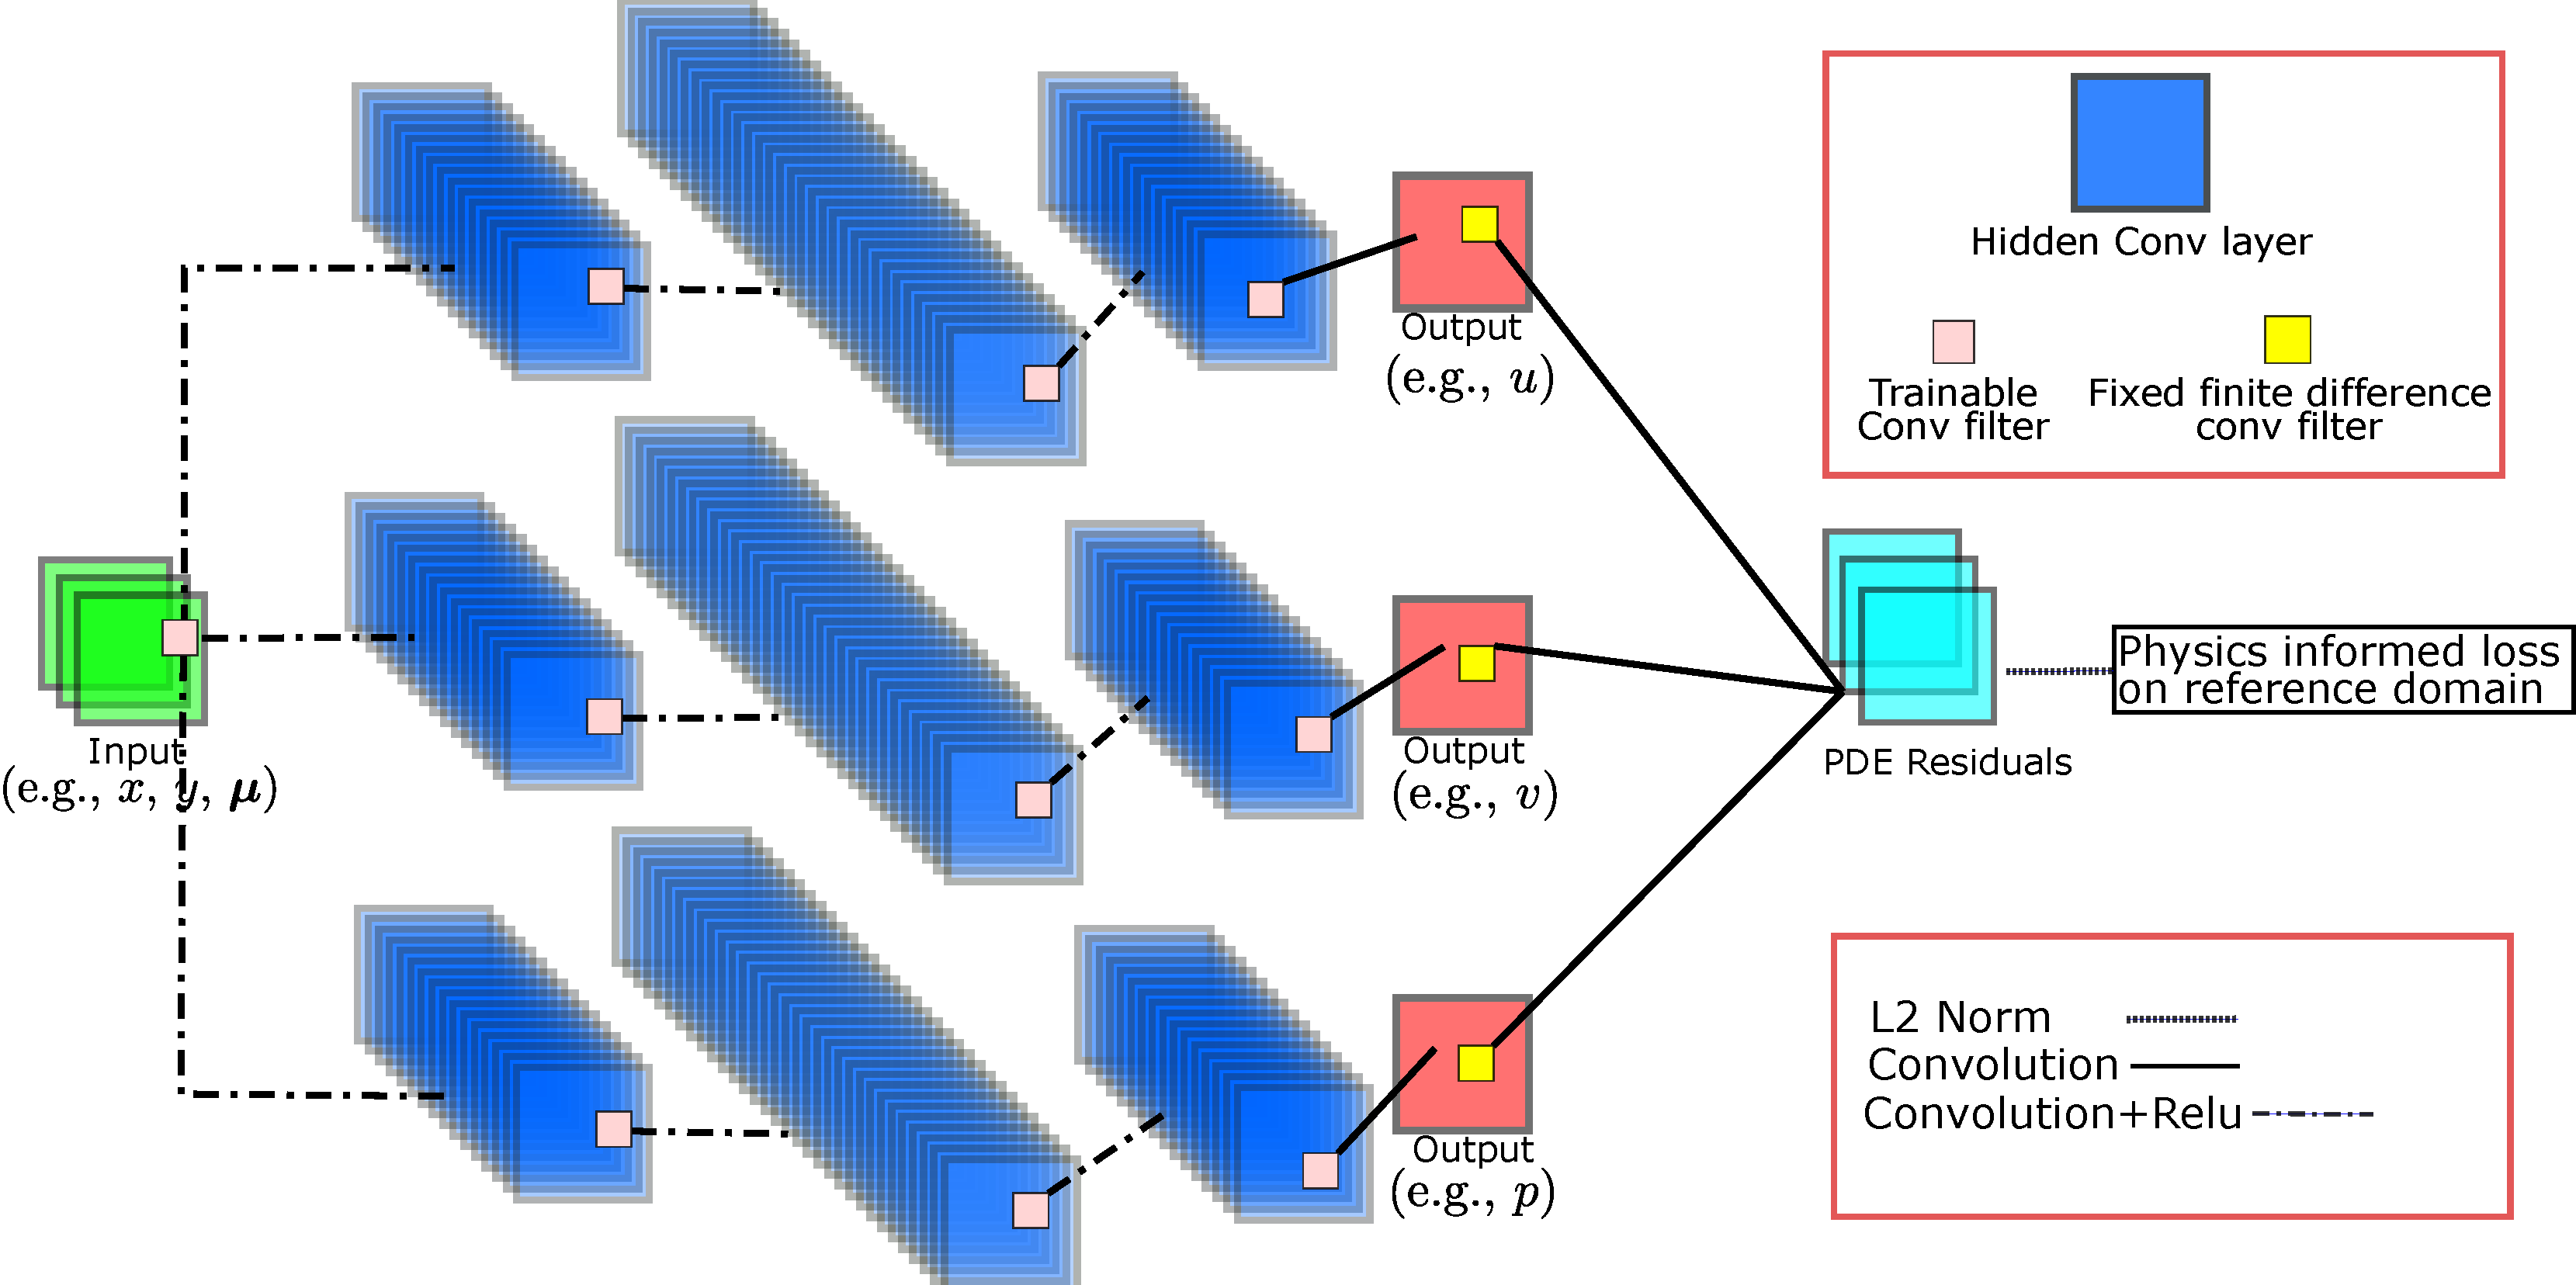
\includegraphics[width=0.7\textwidth]{CNN.pdf}
\vfill
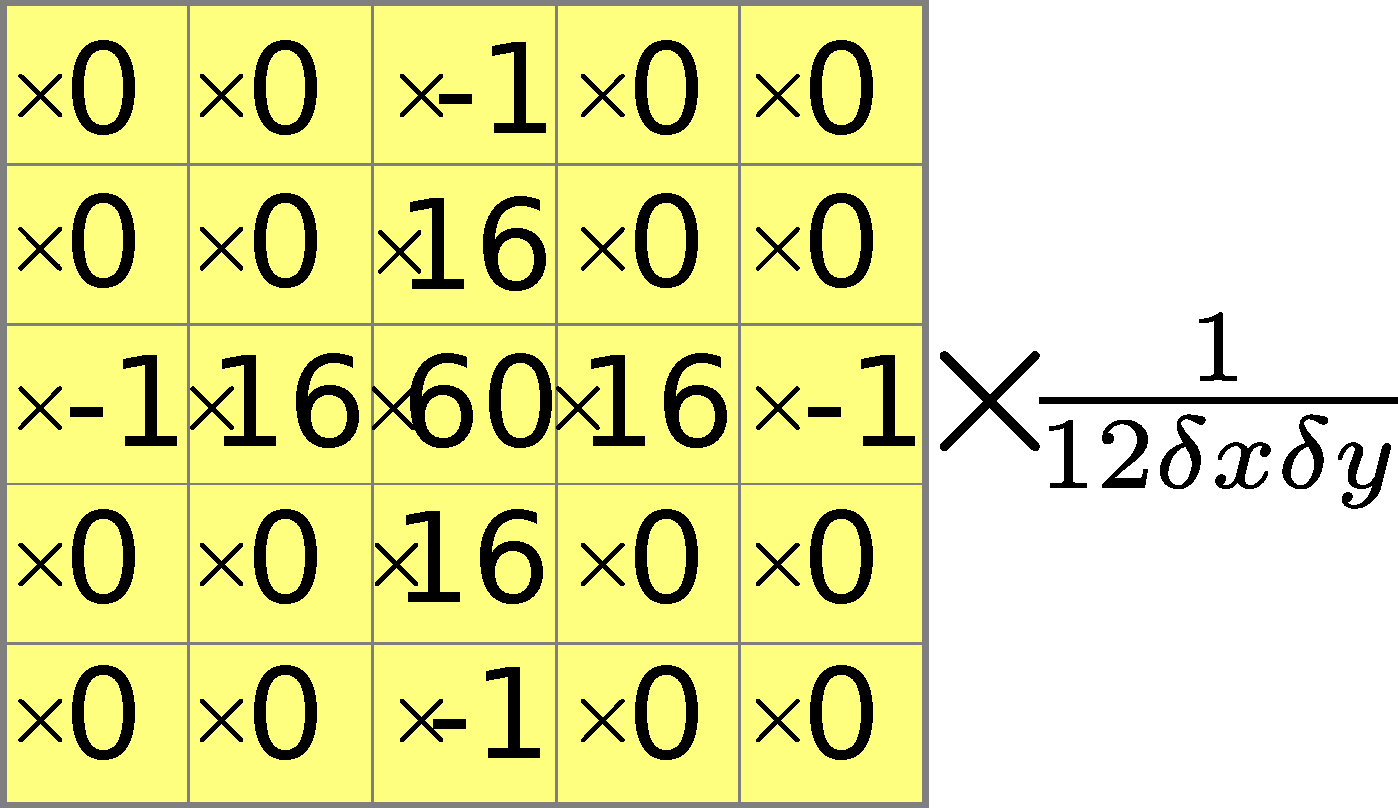
\includegraphics[height=0.2\textwidth]{laplaceU.pdf}
\hfill
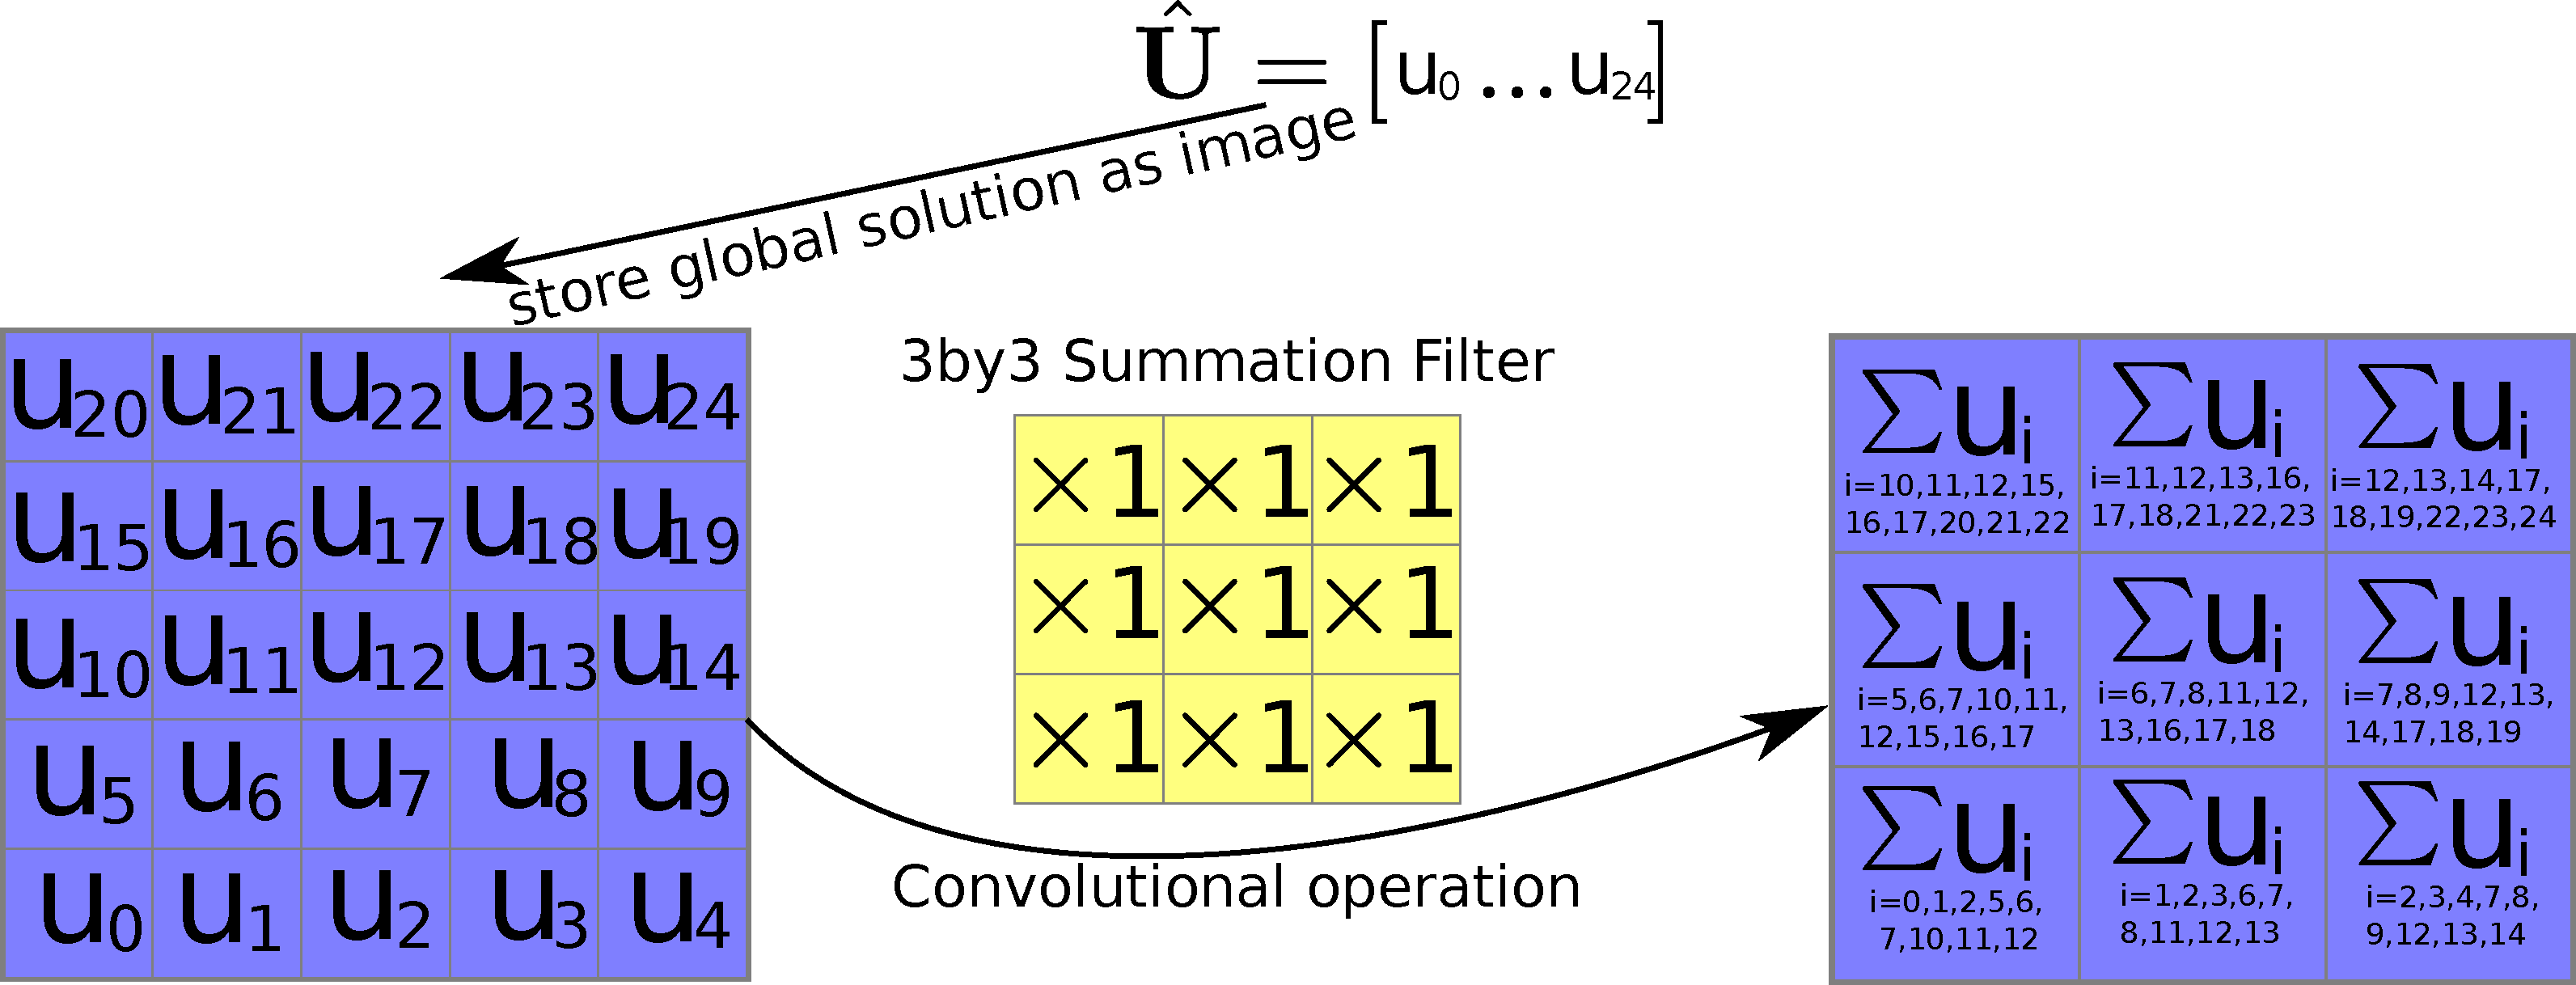
\includegraphics[height=0.2\textwidth]{WhatIsCNN.pdf}
\end{figure}
\end{frame}

\begin{frame}{Deal with irregular domain}
\begin{figure}
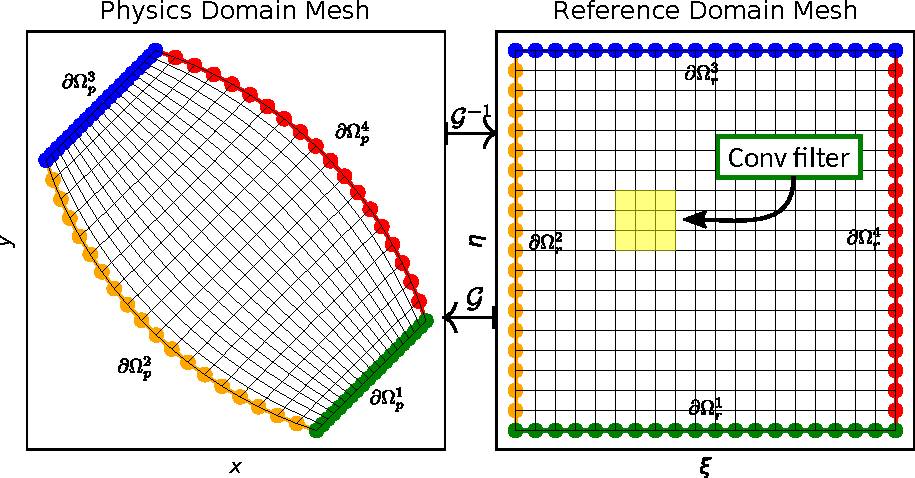
\includegraphics[width=1\textwidth]{PhyGeoCNN}
\end{figure}
\begin{columns}[c]
\column{.5\textwidth}
\begin{equation*}
\xbm=\Gcal(\xibold)\quad \Gcal:\Omega_{r}\mapsto\Omega_{p}
\end{equation*}
\column{.5\textwidth}
\begin{equation*}
\xibold=\Gcal(\xbm)\quad \Gcal^{-1}:\Omega_{p}\mapsto\Omega_{r}
\end{equation*}
\end{columns}
\end{frame}


\begin{frame}{Solve non-linear elliptic PDE to obtain $\Gcal$ and $\Gcal^{-1}$}
\begin{columns}[c]
\column{.3\textwidth}
To obtain $\Gcal^{-1}$, solve:
\tiny
\begin{equation*}
\label{eqn:GInv}
\nabla^2\boldsymbol{\xi}(\mathbf{x}) = 0,
\end{equation*}
\normalsize
To obtain $\Gcal$, solve:
\tiny
\begin{equation*}
	\begin{split}
		\label{eqn:G}
		\alpha\frac{\partial^2x}{\partial\xi^2}-2\beta\frac{\partial^2x}{\partial\xi\partial\beta}+\gamma\frac{\partial^2x}{\partial\eta^2}=0,\\
		\alpha\frac{\partial^2y}{\partial\xi^2}-2\beta\frac{\partial^2y}{\partial\xi\partial\beta}+\gamma\frac{\partial^2y}{\partial\eta^2}=0,
	\end{split}
\end{equation*}
\begin{equation*}
\label{eqn:alphabetagamma}
\begin{split}
\alpha&=\left(\frac{\partial x}{\partial \eta}\right)^2+\left(\frac{\partial y}{\partial \eta}\right)^2,\\
\gamma&=\left(\frac{\partial x}{\partial \xi}\right)^2+\left(\frac{\partial y}{\partial \xi}\right)^2,\\
\beta&=\frac{\partial x}{\partial \xi}\frac{\partial x}{\partial \eta}+\frac{\partial y}{\partial \xi}\frac{\partial y}{\partial \eta}.
\end{split}
\end{equation*}

\column{.7\textwidth}
\pause
What do we gain from this mapping? Directly use backbone of CNN
\pause
\tiny
\begin{equation*}
	\begin{split}
		\label{eqn:Du}
		\frac{\partial }{\partial x}&=\underbrace{\frac{1}{J}}_{\text{constant}}\Big[\left(\frac{\partial }{\partial \xi}\right) \underbrace{\left(\frac{\partial y}{\partial \eta}\right)}_{\text{constant}} - \left(\frac{\partial }{\partial \eta}\right) \underbrace{\left(\frac{\partial y}{\partial \xi}\right)}_{\text{constant}}\Big],\\
		\frac{\partial }{\partial y}&=\underbrace{\frac{1}{J}}_{\text{constant}}\Big[\left(\frac{\partial }{\partial \eta}\right) \underbrace{\left(\frac{\partial x}{\partial\xi}\right)}_{\text{constant}} - \left(\frac{\partial }{\partial \xi}\right) \underbrace{\left(\frac{\partial x}{\partial \eta}\right)}_{\text{constant}}\Big],
	\end{split}
\end{equation*}
\normalsize
\pause
The optimization problem for irregular domain is
\tiny
\begin{equation*}
\label{eqn:optmizationNew}
\begin{split}
&\min_{\Gamma} \sum_{i=1}^{n_d}
\underbrace{\left\|
	\tilde{\mathcal{F}}\Big(\mathbf{u}^{cnn}(\boldsymbol{\Xi}, \boldsymbol{\mu}_i; \Gamma),
	\nabla\mathbf{u}^{cnn}(\boldsymbol{\Xi}, \boldsymbol{\mu}_i; \Gamma), 
	\nabla^2\mathbf{u}^{cnn}(\boldsymbol{\Xi}, \boldsymbol{\mu}_i; \Gamma), \cdots; \boldsymbol{\mu}_i\Big) \right\|_{\Omega_{r}}}_{\text{equation-based loss on reference domain:}\ \tilde{\mathcal{L}}_{pde}},\\
&s.t.\;\; \tilde{\mathcal{B}}\Big(\mathbf{u}^{cnn}(\boldsymbol{\Xi}, \boldsymbol{\mu}_i; \Gamma),
\nabla\mathbf{u}^{cnn}(\boldsymbol{\Xi}, \boldsymbol{\mu}_i; \Gamma), 
\nabla^2\mathbf{u}^{cnn}(\boldsymbol{\Xi}, \boldsymbol{\mu}_i; \Gamma), \cdots;
\boldsymbol{\mu}_i\Big)=0,\;\;\text{on }\partial\Omega_{r}.
\end{split}
\end{equation*} 
\end{columns}
\end{frame}


%------------------------------------------------
\section{Result}

\begin{frame}
\frametitle{Result on regular domain}
\begin{figure}
	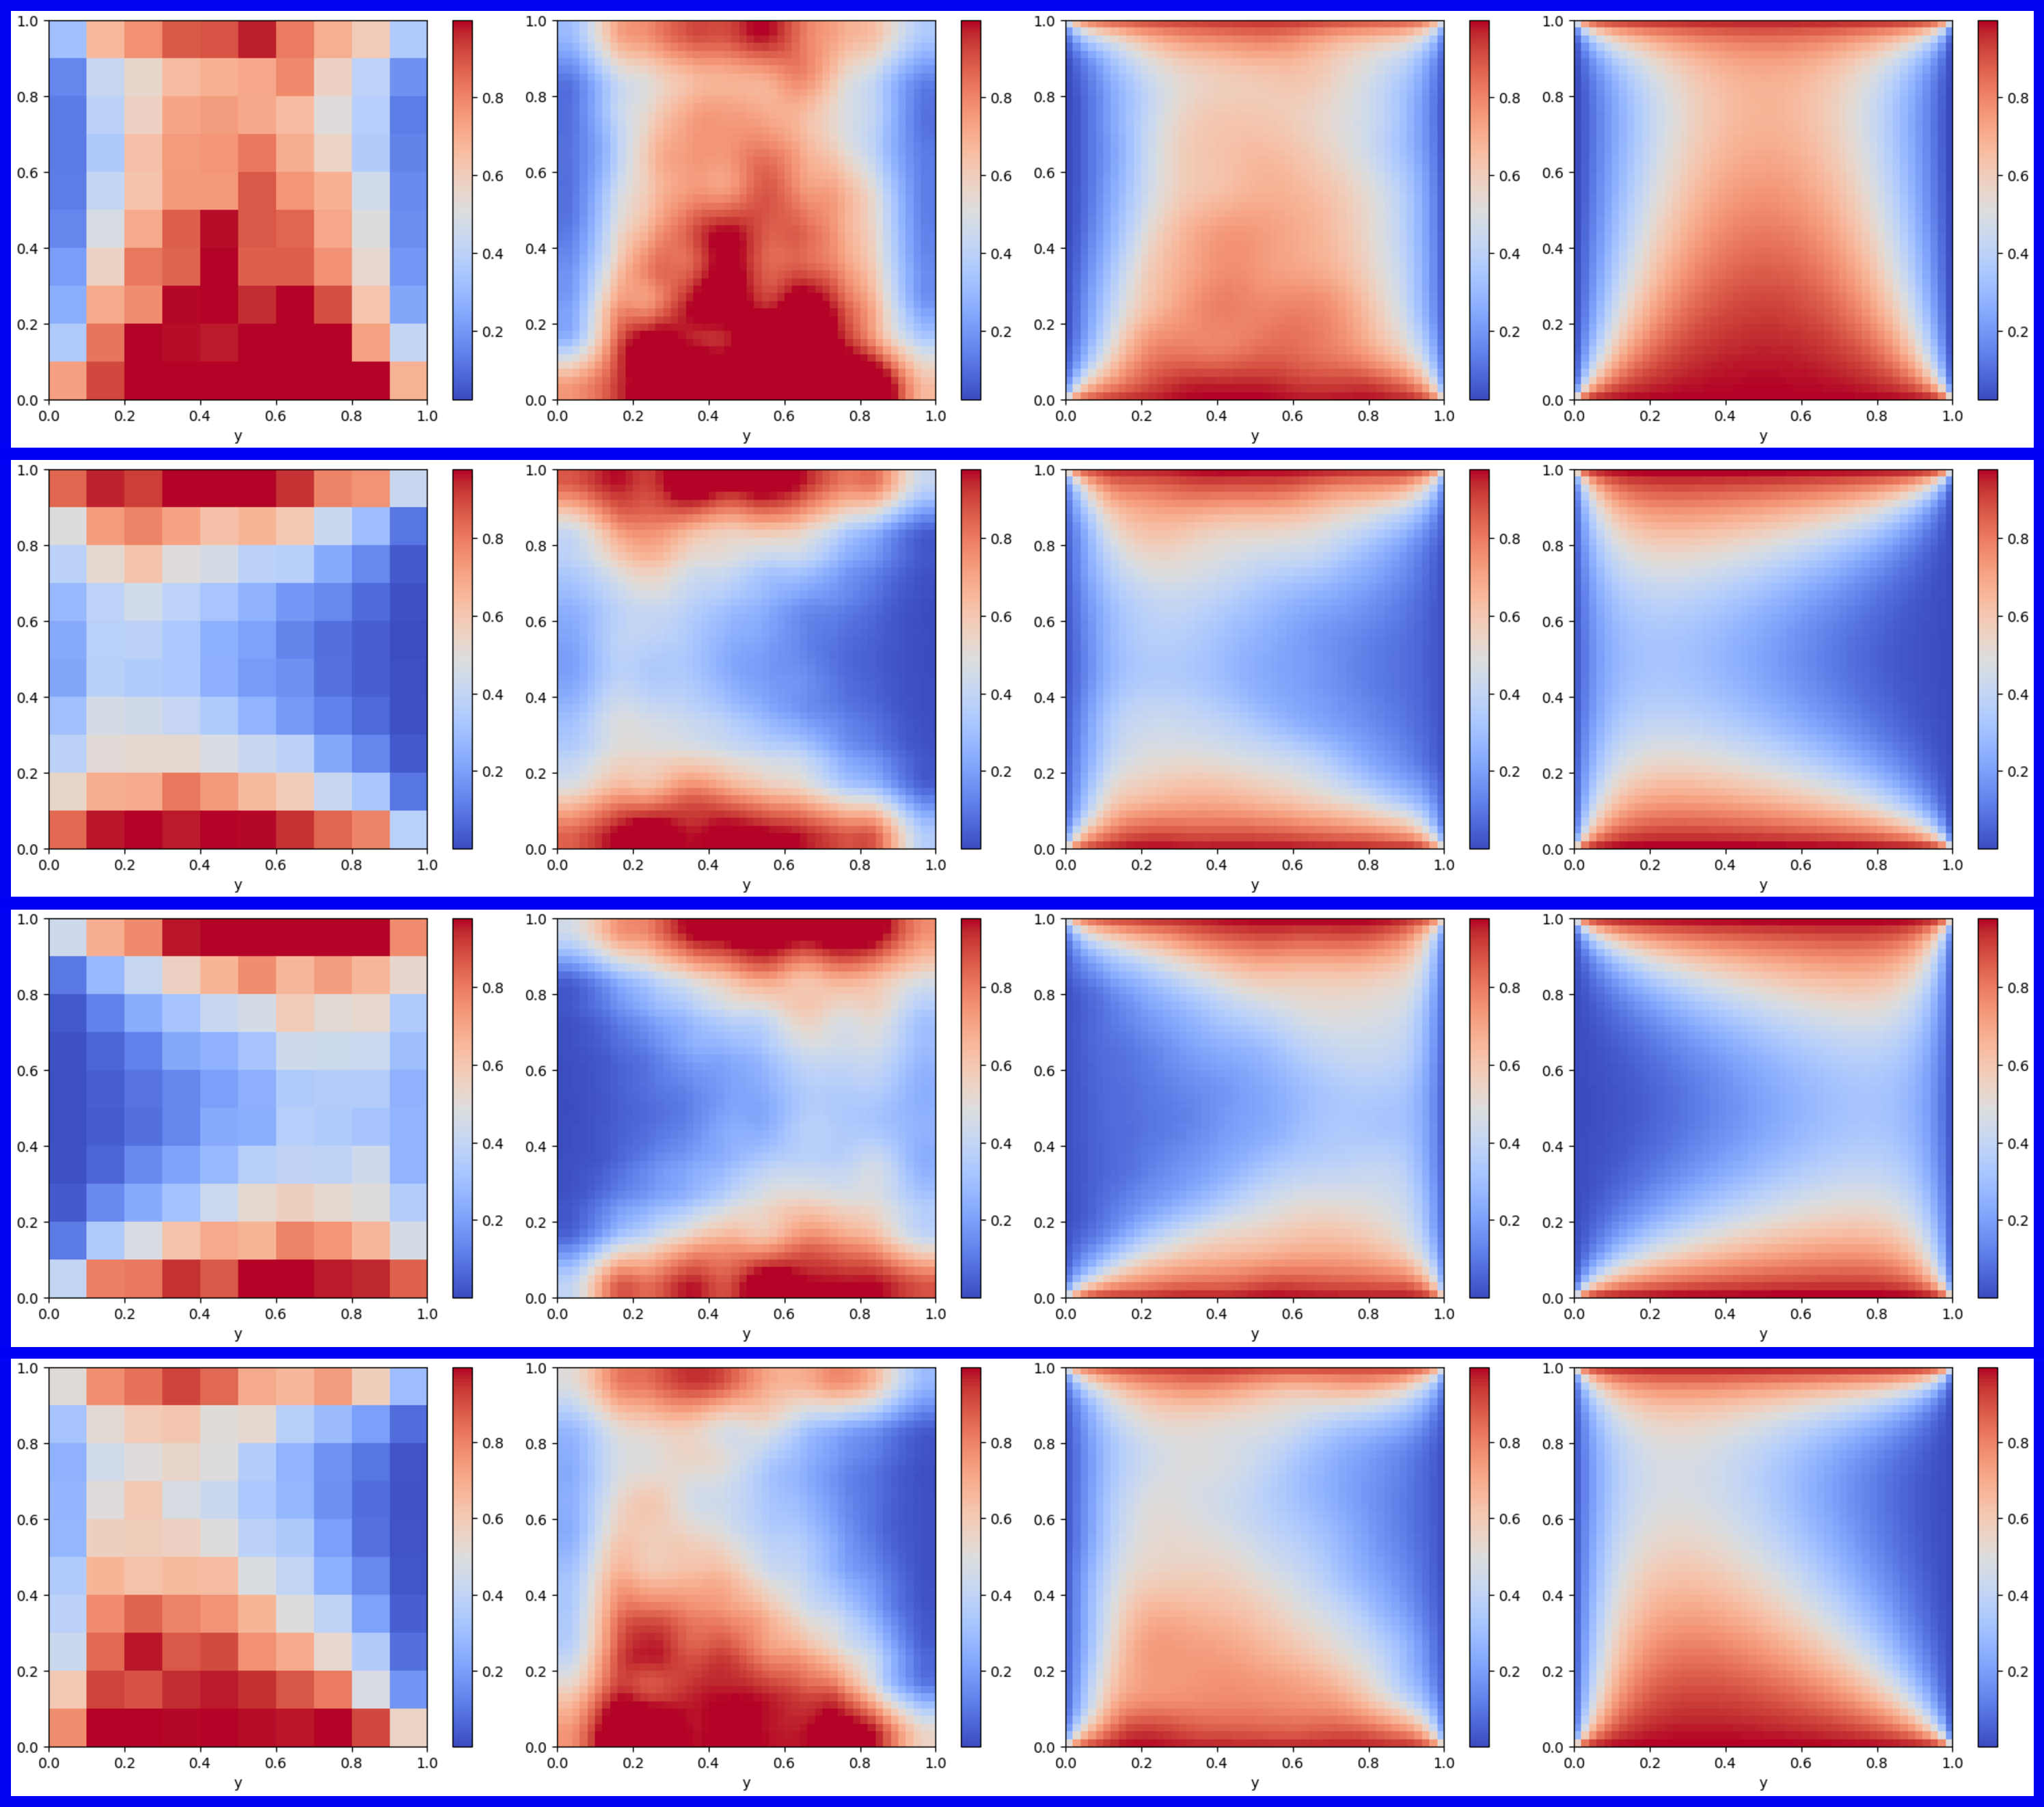
\includegraphics[height=0.4\textwidth]{covecdiffpdf.pdf}
	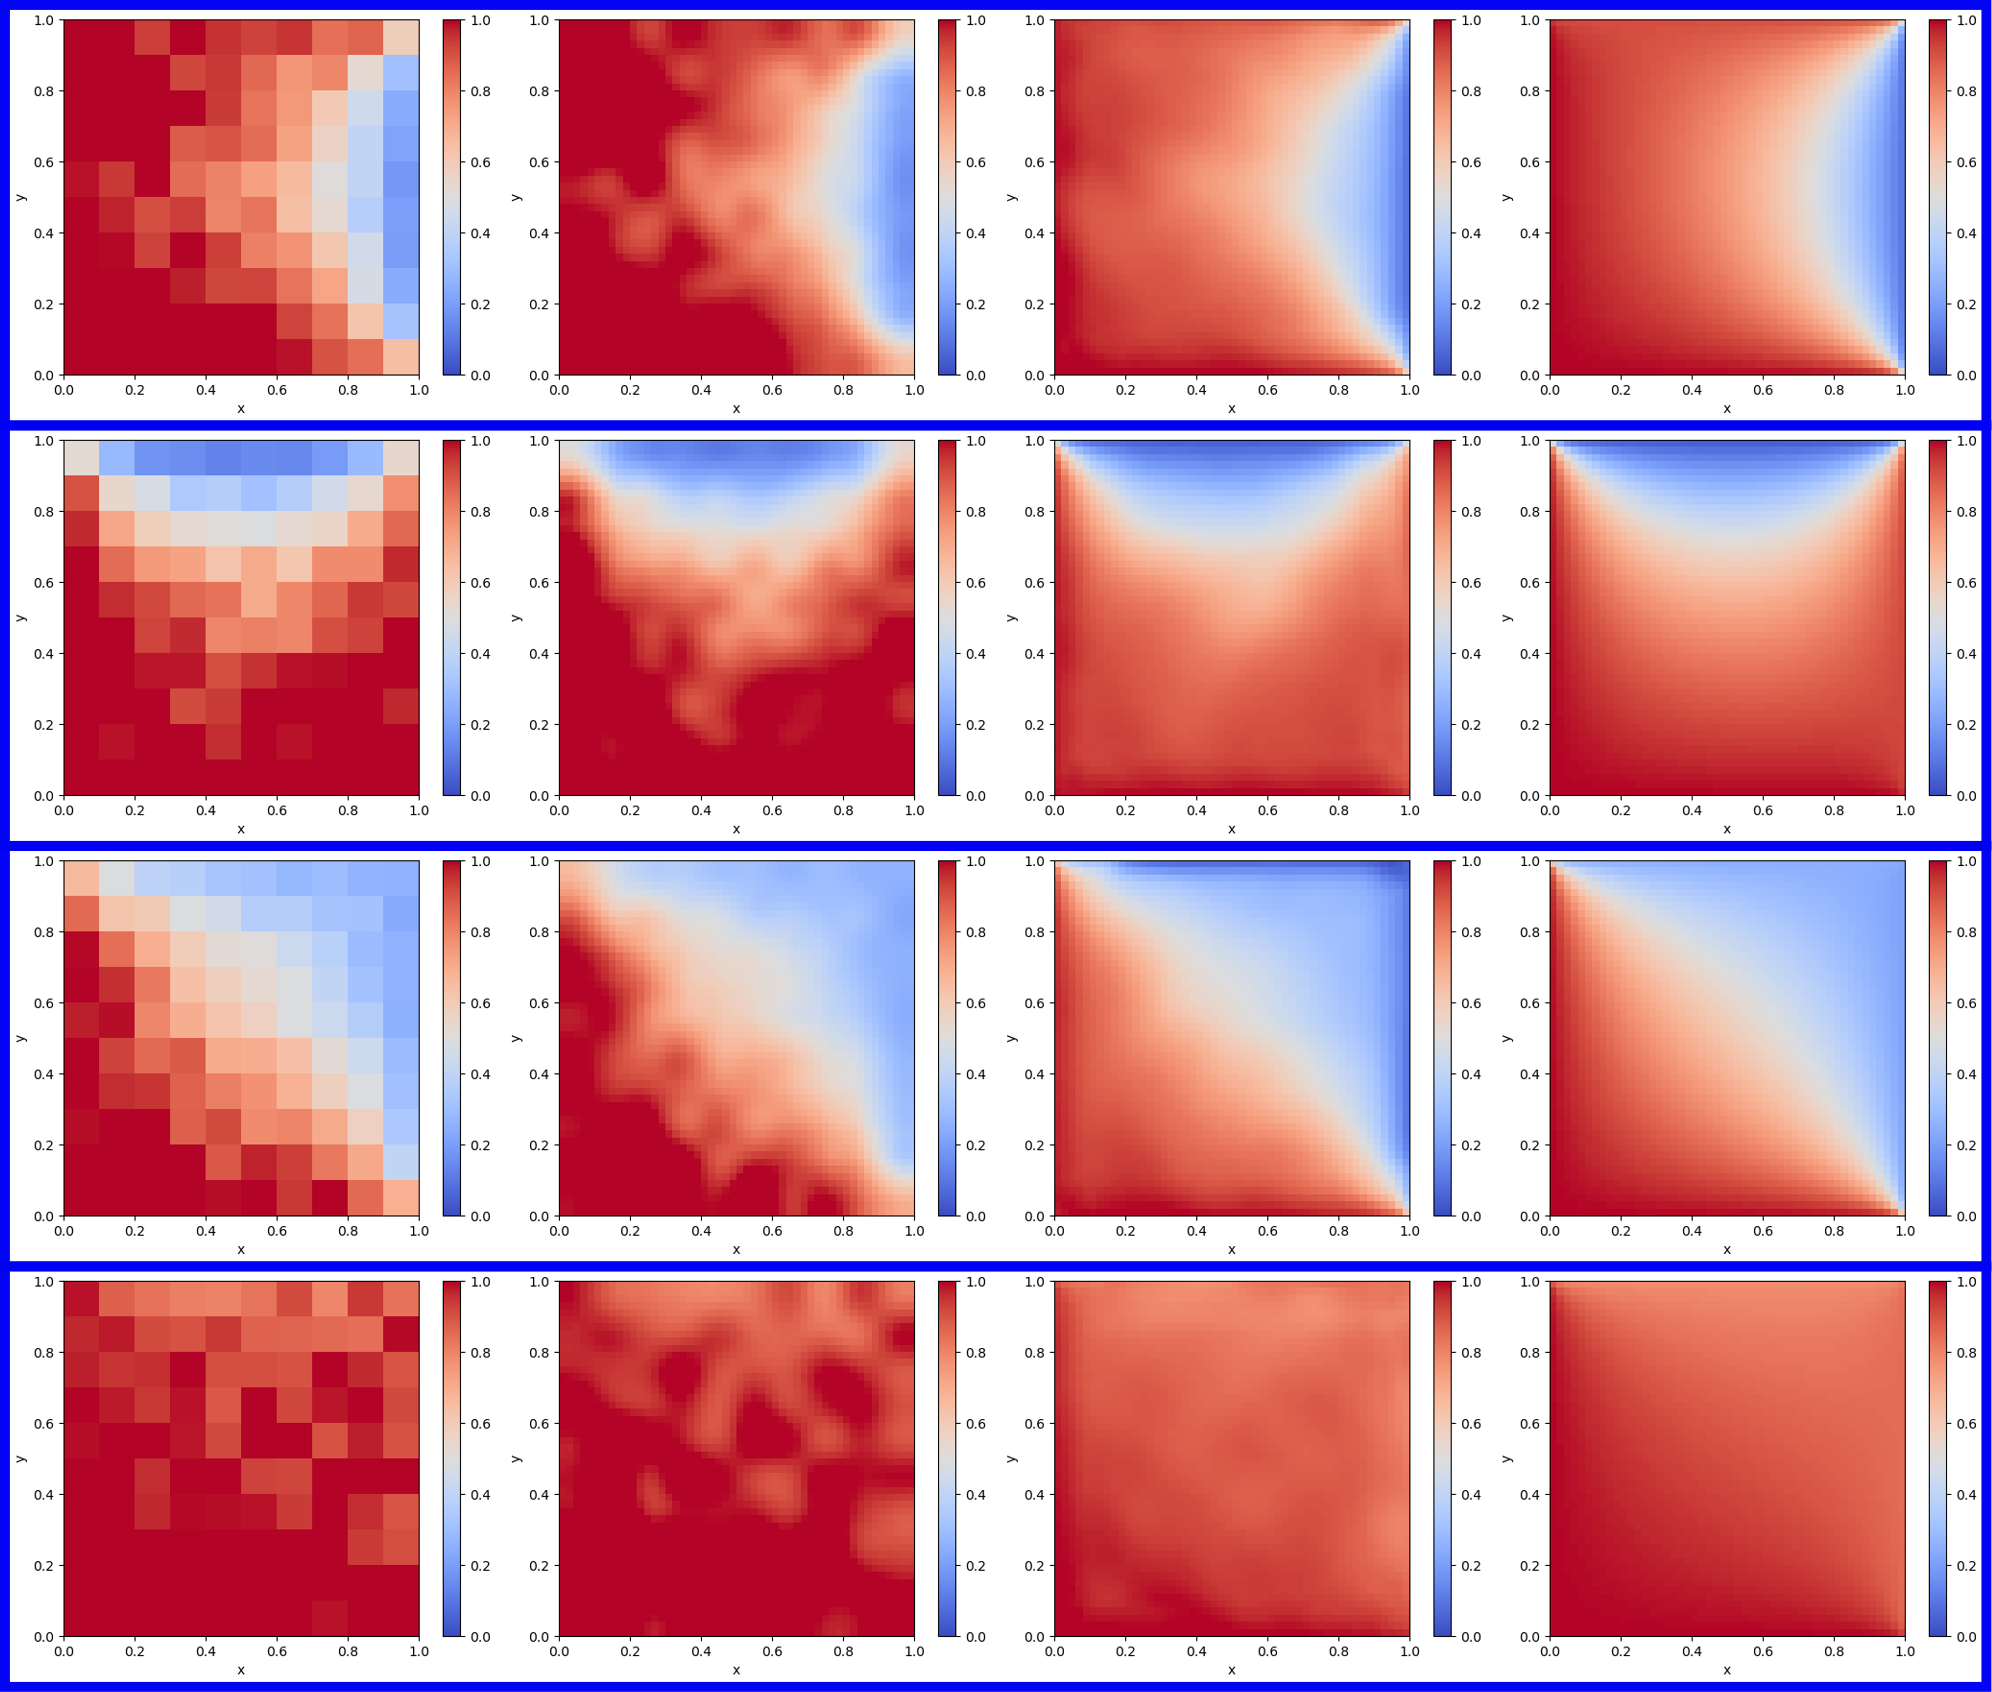
\includegraphics[height=0.4\textwidth]{Heat.png}
\end{figure}
Convection diffusion equation (left) and heat equation (right).
\end{frame}

\begin{frame}{Result on irregular domain}
\begin{columns}[c] % The "c" option specifies centered vertical alignment while the "t" option is used for top vertical alignment
\column{0.5\textwidth} % Right column and width
\begin{figure}
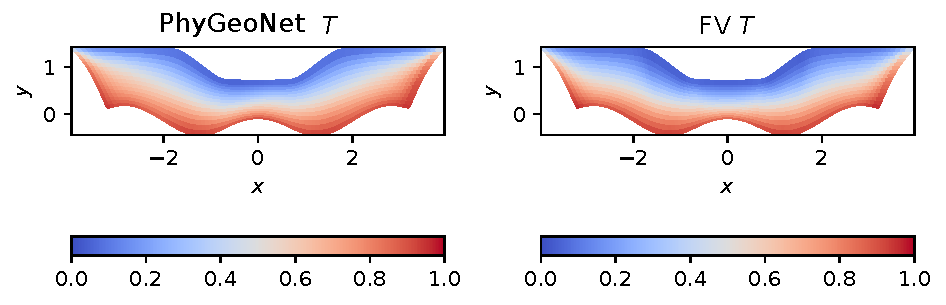
\includegraphics[width=1\textwidth]{DetHeat_1274T.pdf}
\vfill
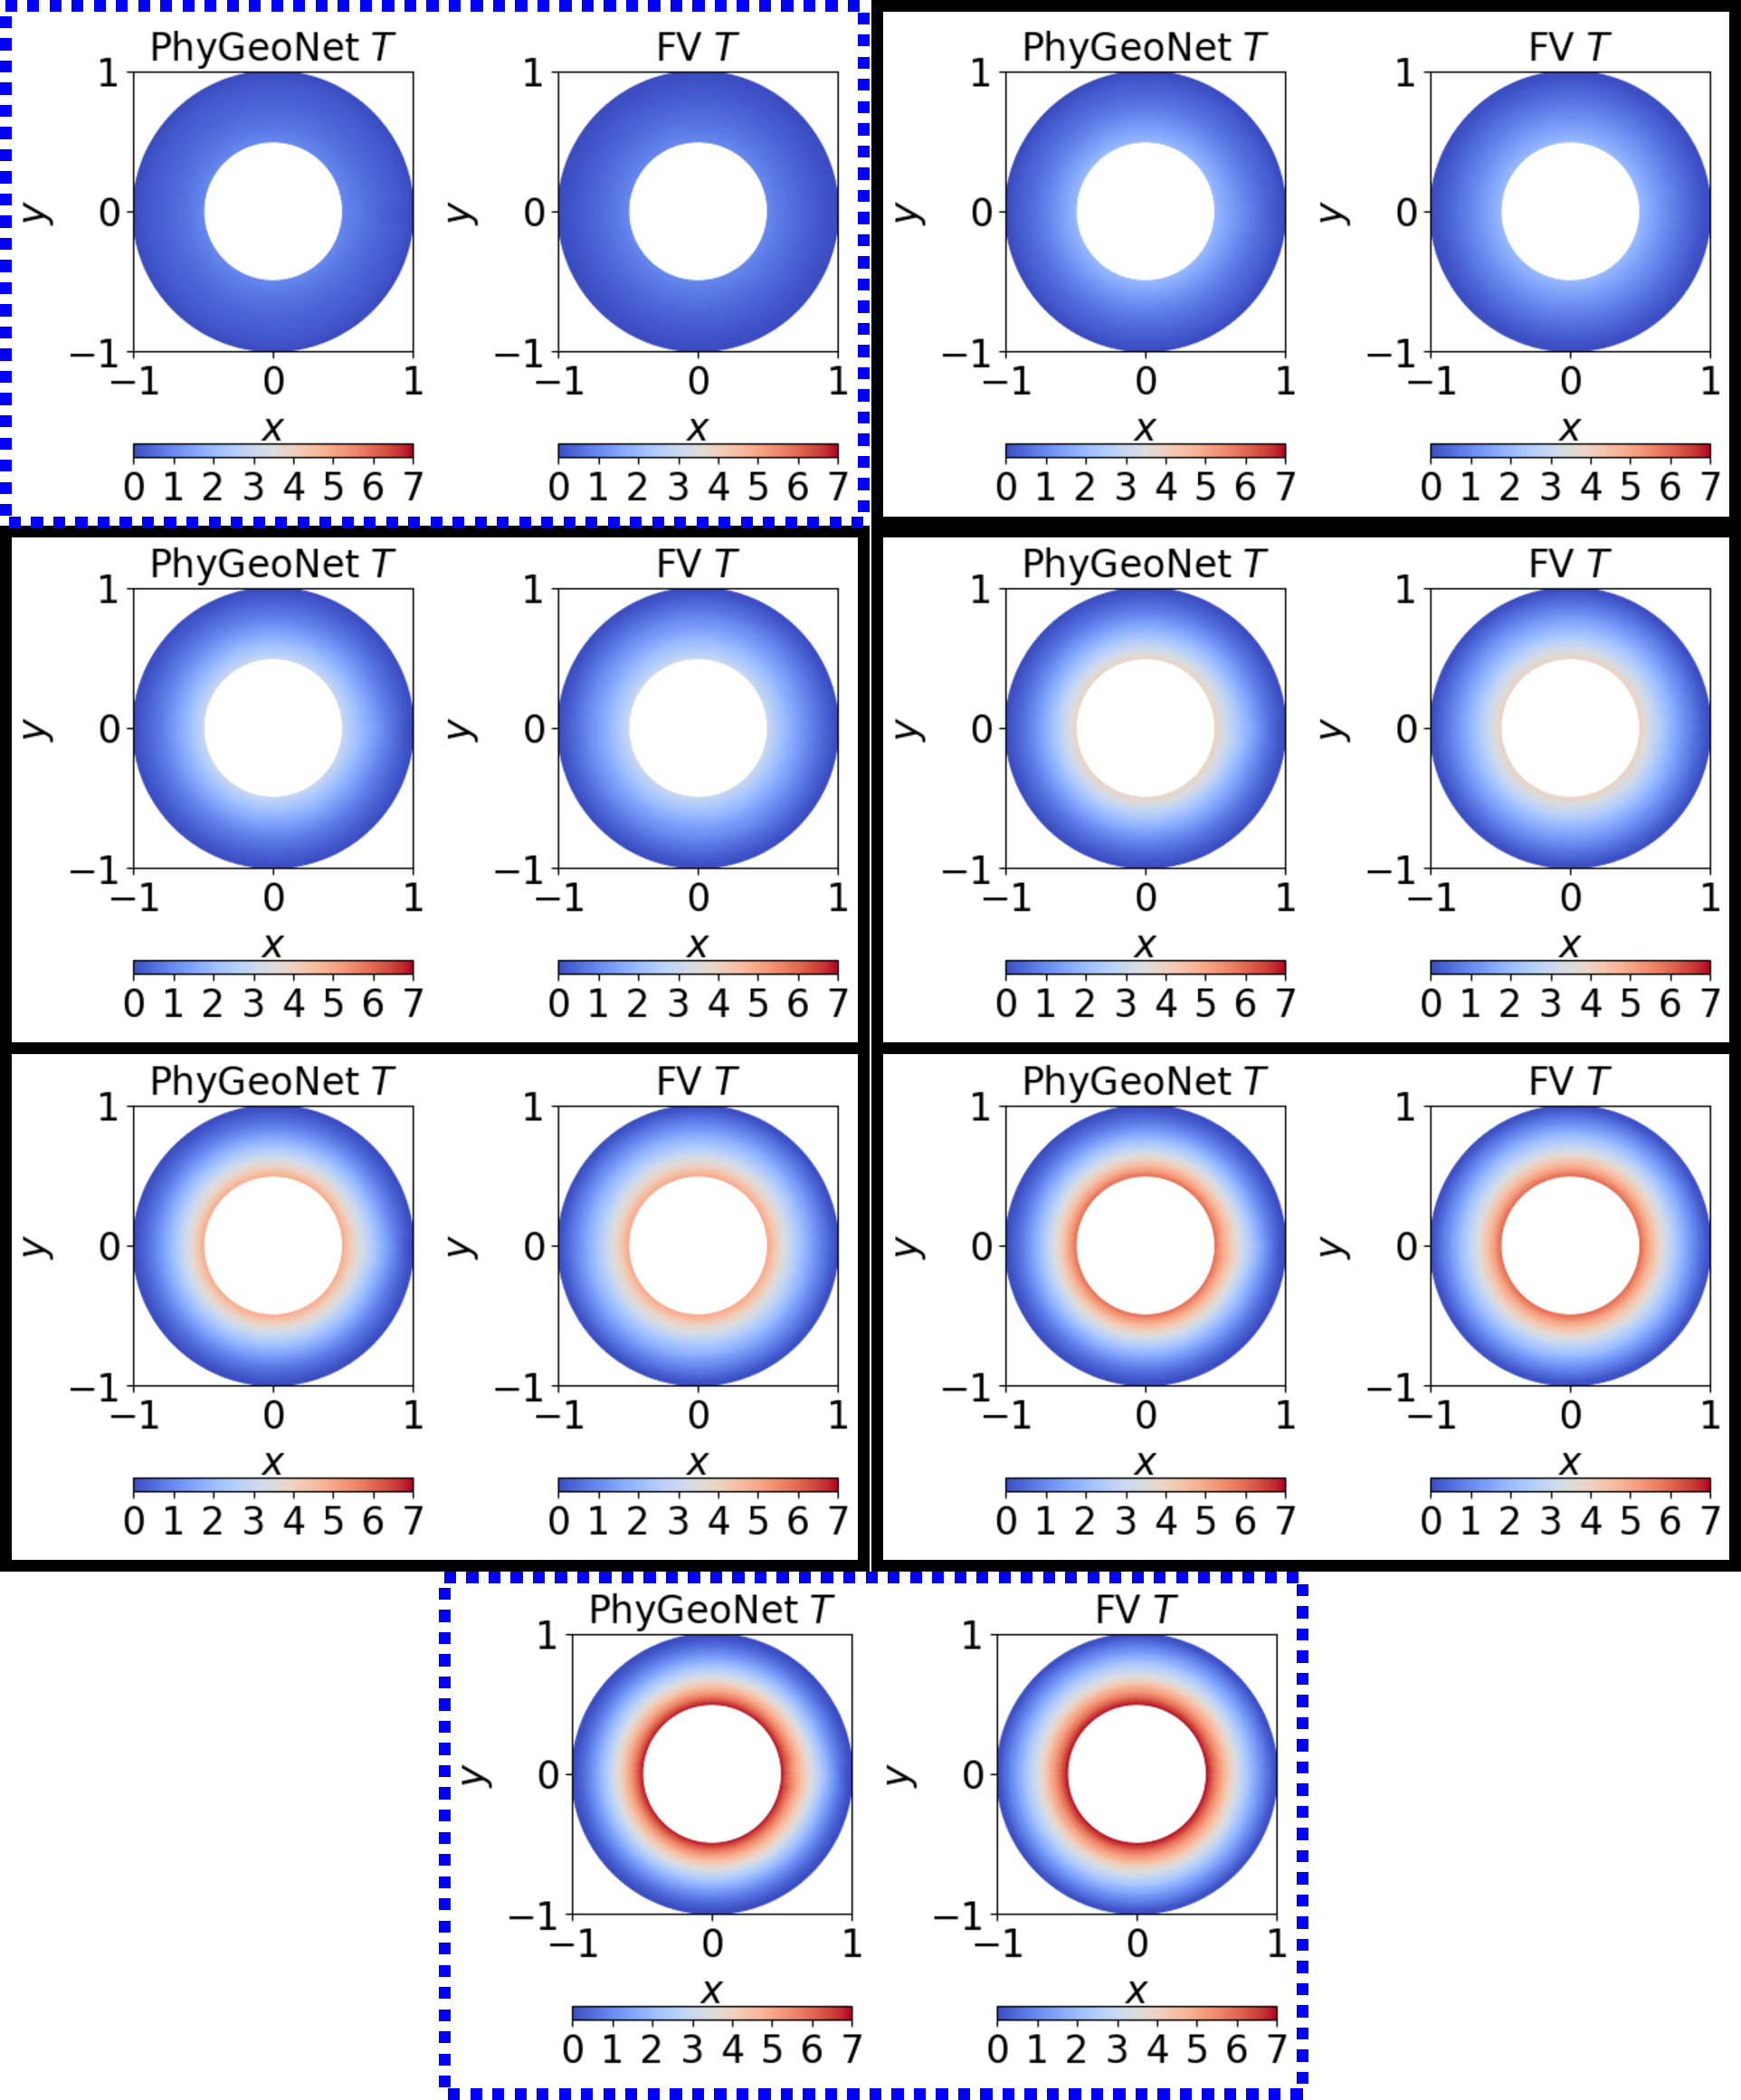
\includegraphics[width=0.6\textwidth]{ParaHeat_Contour.pdf}
\end{figure}
\centering
Heat equation

\column{0.5\textwidth} % Right column and width
\begin{figure}
	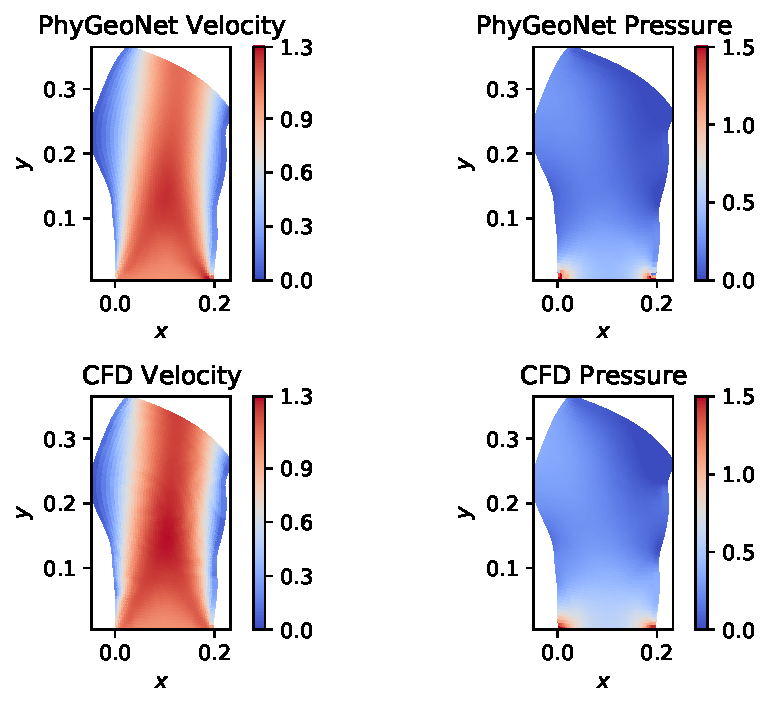
\includegraphics[width=0.5\textwidth]{DetNS_15000VelMagAndPressure.pdf}
	\vfill
	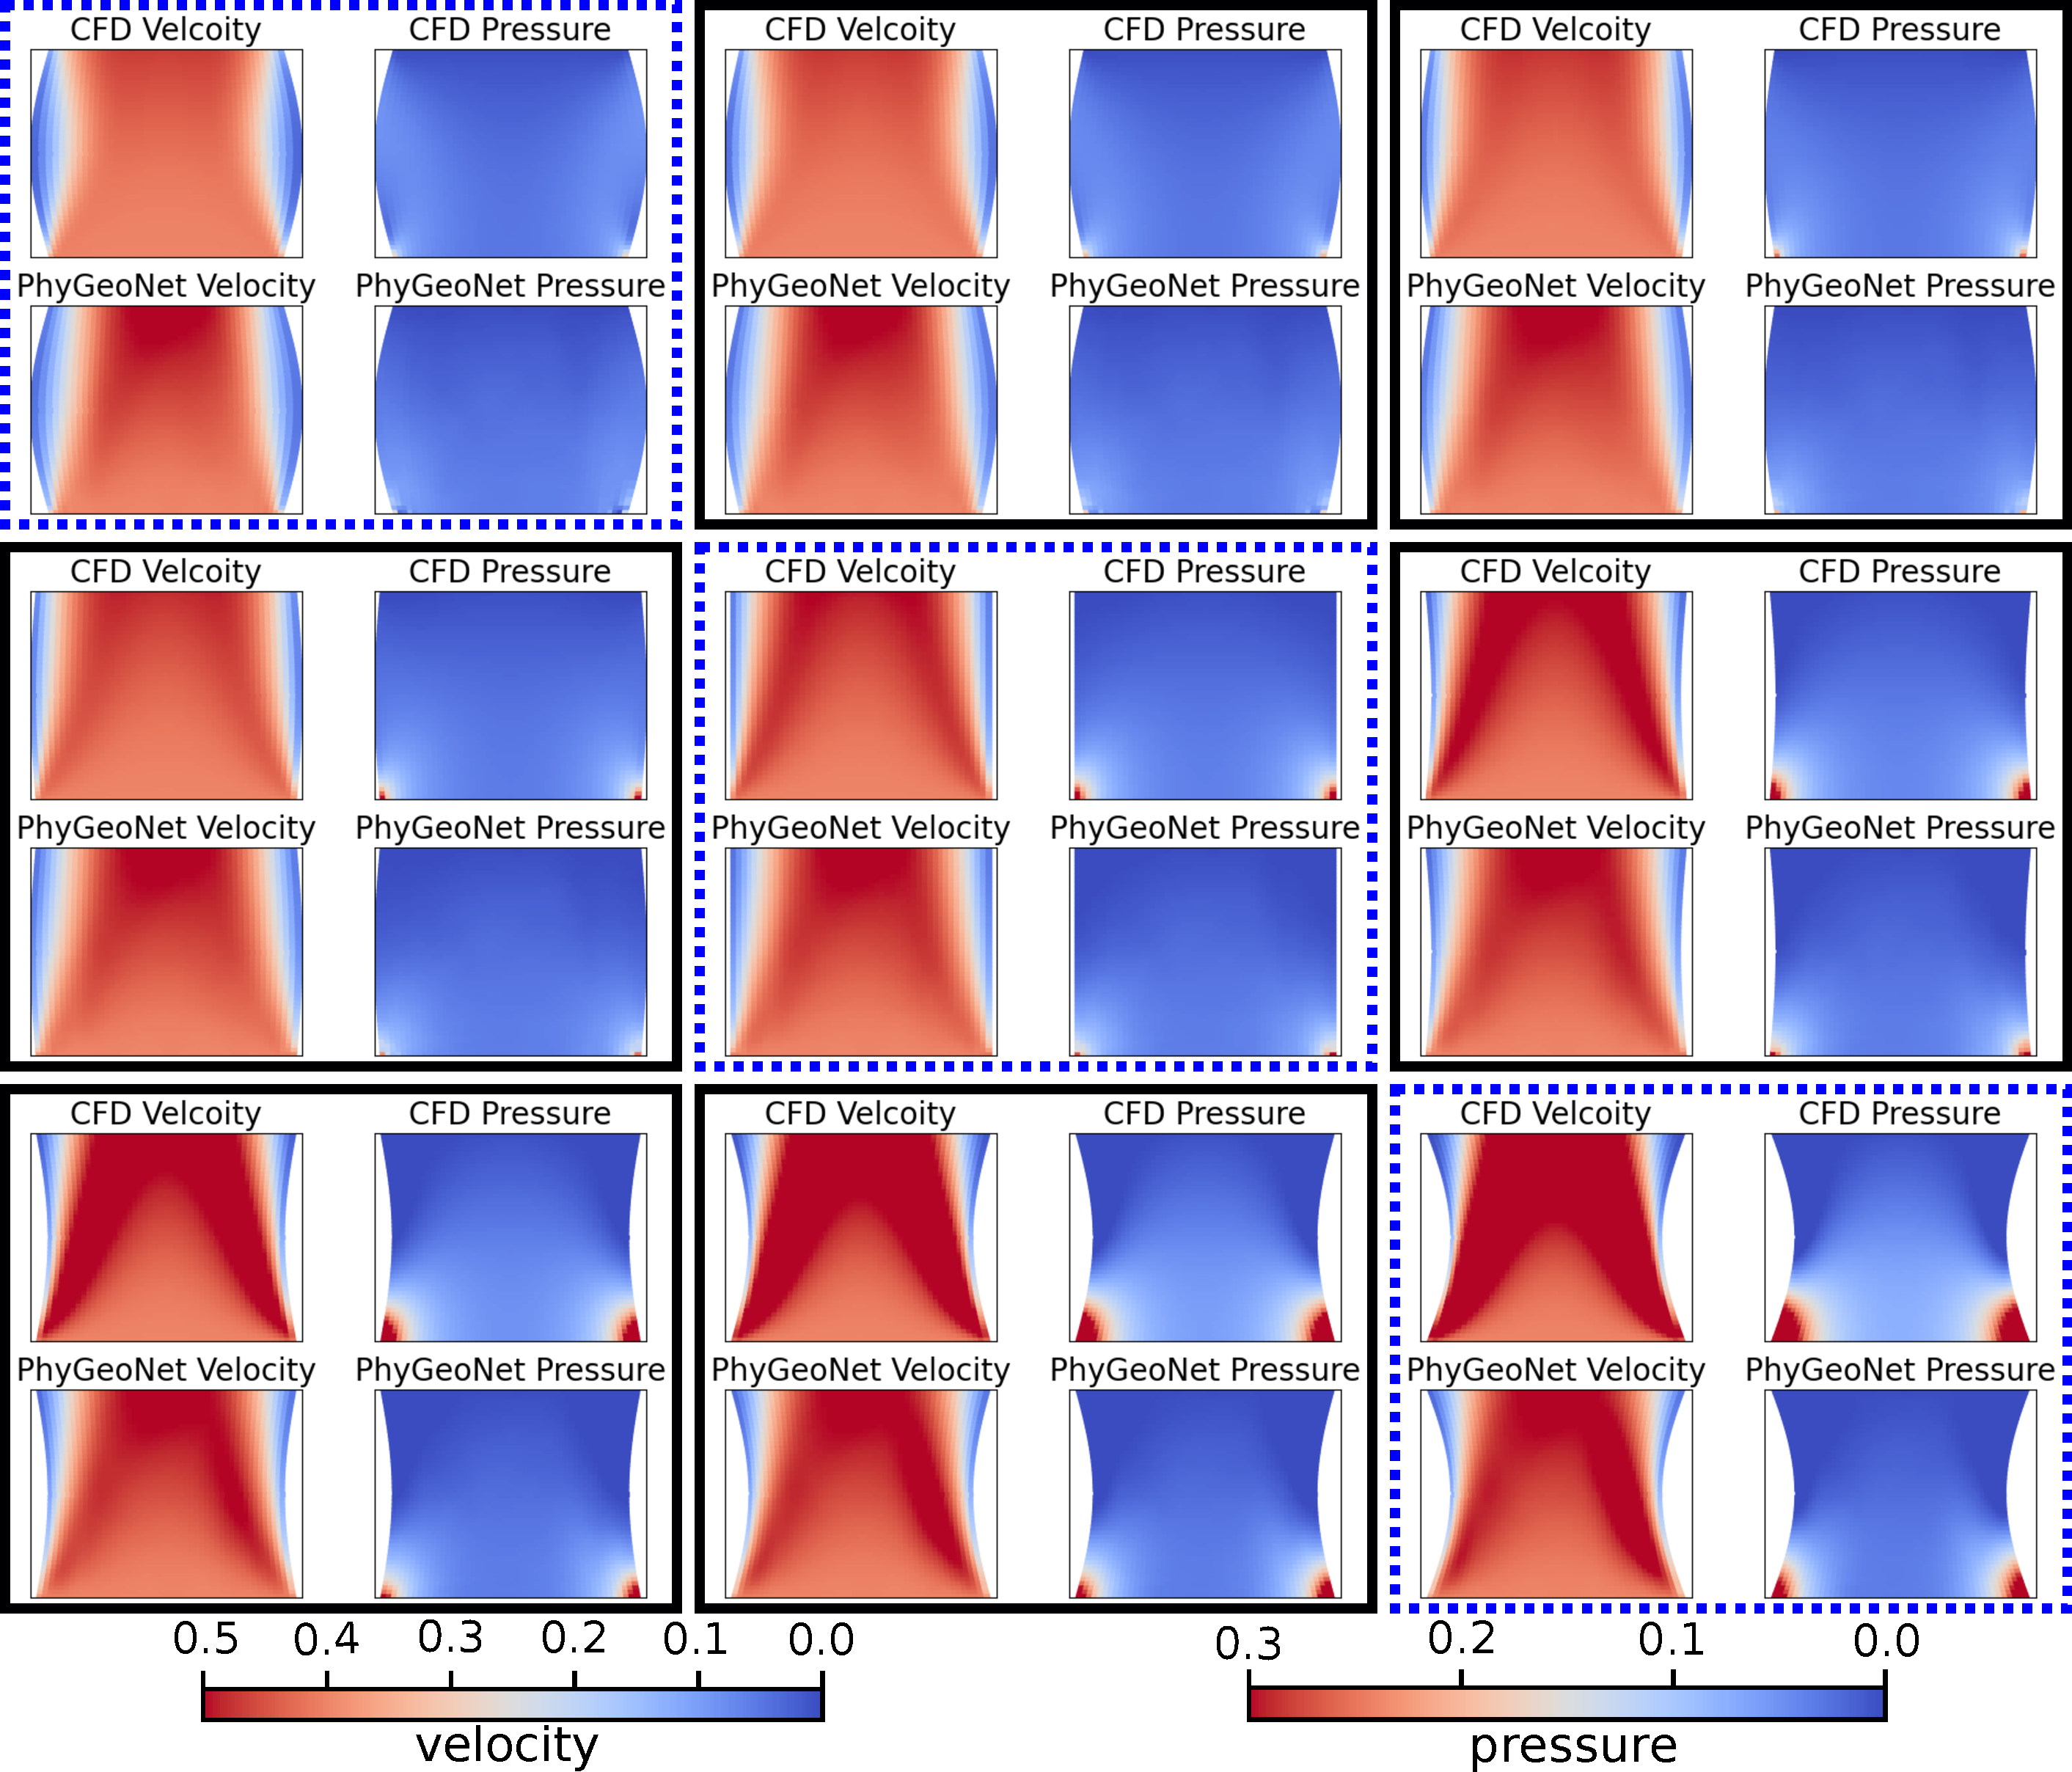
\includegraphics[width=0.6\textwidth]{ParaNS_ResultContour.pdf}
\end{figure}
\centering
NS equation
\end{columns}
\end{frame}
%------------------------------------------------

%------------------------------------------------

\begin{frame}{Reference}
Gao, Han, Luning Sun, and Jian-Xun Wang. "PhyGeoNet: Physics-Informed Geometry-Adaptive Convolutional Neural Networks for Solving Parametric PDEs on Irregular Domain." arXiv preprint arXiv:2004.13145 (2020).
\end{frame}
%------------------------------------------------

\begin{frame}{Acknowledgment}
\begin{itemize}
	\item Thanks to my adviser, Jian-Xun Wang
	\item Thanks to Dr. Lu Lu and Prof. George Em Karniadakis for giving me this opportunity to share my work with people in this area.
	\item Thanks for all the speakers and audience, I learn a lot from everybody in this symposium.
\end{itemize}
\end{frame}

%----------------------------------------------------------------------------------------

\end{document} 